%----------------------------------------------------------------
%
%  File    :  thesis.tex
%
%  Author  :  Keith Andrews, ISDS, TU Graz, Austria
%
%  Created :  30 Jul 1997
% 
%  Changed :  22 Jan 2021
%
%----------------------------------------------------------------

\documentclass[11pt]{book}
\usepackage[
  a4paper,
  twoside,
  top=5mm,                % top margin
  bottom=7mm,             % bottom margin
  inner=20mm,             % inner margin (next to binding)
  outer=20mm,             % outer margin (opposite binding)
  bindingoffset=10mm,     % on binding side
  includeheadfoot,        % include head(er) and foot(er)
  headheight=10mm,        % height of header
  headsep=15mm,           % sep between header and text body
  footskip=15mm,          % sep between body and baseline of footer
  footnotesep = 10mm plus 2mm minus 0mm  % bottom of body to top of footnote
]{geometry}
% A4 paper is w=210m, h=297mm


\newcommand{\thisdate}{03 Dec 2021}  % date of this version
\newcommand{\thisyear}{2021}         % year of this version


\newcommand{\fullh}{24cm}         % height of figures for 1 per page
\newcommand{\halfh}{9.5cm}        % height of figures for 2 per page
\newcommand{\thirdh}{6cm}         % height of figures for 3 per page


\setlength{\parindent}{1em}       % less indentation
\setlength{\parskip}{1.5ex plus 0.3ex minus 0.3ex}  % vert. space before para


% \tolerance is set by LaTeX to 200
% \sloppy sets \tolerance = 9999
% which allows LaTeX more tolerance in adding word spacing

% \sloppy
% \fussy
% \tolerance = 1000

\tolerance=400 
% makes some lines with lots of white space, but      
% tends to prevent words from sticking out in the margin



\setcounter{secnumdepth}{3}     % lowest section level still numbered
\setcounter{tocdepth}{2}        % lowest section level entered in ToC




\usepackage[T1]{fontenc}        % 8-bit output chars (must be before inputenx)
\usepackage[utf8]{inputenx}     % input char encoding

\usepackage[english,austrian,british]{babel}

\usepackage{newtxtext}          % newer times fonts
\usepackage{newtxmath}

\usepackage{relsize}            % relative font sizes \smaller \larger
\usepackage{float}              % H for float placement
\usepackage{setspace}           % adjust line spacing

\usepackage{textcomp}           % symbols such as \texttimes and \texteuro
\usepackage{latexsym}
\usepackage{fontawesome}        % fontawesome symbols

\usepackage{siunitx}            % prettier number formatting
\sisetup{%
  group-separator={,},
  group-minimum-digits=4,
}
\usepackage[super]{nth}         % 1st, 2nd, 3rd, etc.

\usepackage{xspace}
\usepackage{xstring}            % string manipulation macros
\usepackage{xparse}             % commands with optional arguments
\usepackage{etoolbox}           % for \newrobustcmd
\usepackage{makecmds}           % for \makecommand
\usepackage{calc}               % for math calculations


\usepackage[svgnames,table,xcdraw]{xcolor}
\definecolor{darkgreen}{rgb}{0.0,0.2,0.0}
\definecolor{darkblue}{rgb}{0.0,0.0,0.2}
\definecolor{darkred}{rgb}{0.2,0.0,0.0}
\definecolor{verylightgrey}{gray}{0.95}
\definecolor{lightgrey}{gray}{0.9}
\definecolor{grey}{gray}{0.7}
\definecolor{black}{gray}{0.0}

\definecolor{tableheadercolour}{gray}{0.8}
\definecolor{tablerowcolour}{gray}{0.93}




\usepackage{longtable}
\usepackage{multirow}
\usepackage{tabularx}

% Define some new column types for tables:
% like X but flushleft (= raggedright) rather than justified
\newcolumntype{Y}{>{\raggedright\arraybackslash}X}
% a p column but flushleft (= raggedright) rather than justified
\newcolumntype{L}[1]{>{\raggedright\arraybackslash}p{#1}}
% a p column but flushright (= raggedleft) rather than justified
\newcolumntype{R}[1]{>{\raggedleft\arraybackslash}p{#1}}


\usepackage{booktabs}           % nicer tables

\newcommand{\tablestretch}
{\renewcommand{\arraystretch}{1.20}}  % spacing between table rows




\usepackage{verbdef}            % define robust verb strings
\usepackage{verbatim}
\usepackage{comment}



% better lists
\usepackage{enumitem}

\setlist{
  topsep=0pt,
  partopsep=0pt,
  parsep=0.6ex,
  itemsep=1.2ex,
  left=\parindent .. 2\parindent,    % bullet .. start ot text
}

\setlist[description]{
  style=sameline,
}




\usepackage{listings}                 % for listings of source code

\makeatletter
\newlength{\numwidth}%
\setlength{\numwidth}{\widthof{\normalfont{\lst@numberstyle{99}}}}% Up to 2-digit (99) line numbers
\def\lst@PlaceNumber{%
  \makebox[\numwidth+1em][l]{%
    \makebox[\numwidth][r]{\normalfont\lst@numberstyle{\thelstnumber}}%
  }%
}
\makeatother

% lstset strategy: define defaults here for
% all non-floating (displayed) listings
% floated listings override these settings later

\lstset{                              % set parameters for listings
  floatplacement=tp,                  % default float placement
  numberbychapter,
  inputencoding=utf8,
  language=,                          % empty = plain text
  tabsize=2,
  xleftmargin=2\parindent,
  xrightmargin=2\parindent,
  frame=none,
  framexleftmargin=0mm,
  rulesepcolor=\color{verylightgrey},
  numbers=none,
  numberstyle=\scriptsize,
  numbersep=2ex,
  breaklines,
  showtabs=false,
  showspaces=false,
  showstringspaces=false,
  %
  basicstyle=\small\ttfamily,
  keywordstyle=\color{black},
  identifierstyle=\color{black},
  commentstyle=\color{SteelBlue},
  stringstyle=\color{DarkOrange},
  %
  captionpos=b,
  abovecaptionskip=\abovecaptionskip,
  belowcaptionskip=\belowcaptionskip,
  extendedchars=true,
  literate=%
    { }{{~}}1
    {©}{{\textcopyright}}1
    {€}{{\texteuro}}1
    {Ö}{{\"O}}1
    {Ä}{{\"A}}1
    {Ü}{{\"U}}1
    {ß}{{\ss}}1
    {ö}{{\"o}}1
    {ä}{{\"a}}1
    {ü}{{\"u}}1,       % map some utf8 chars for listings
}


\lstdefinelanguage{biblatex}   % based on biblatex v 2.7a from 2013-07-14
{
  keywords={%
    @article,@book,@mvbook,@inbook,@bookinbook,@suppbook,%
    @booklet,@collection,@mvcollection,@incollection,@suppcollection,%
    @manual,@misc,@online,@patent,@periodical,@suppperiodical,%
    @proceedings,@mvproceedings,@inproceedings,@reference,@mvreference,%
    @inreference,@report,@set,@thesis,@unpublished,@xdata,%
    @conference,@electronic,@mastersthesis,@phdthesis,@techreport,@www,%
    @artwork,@audio,@bibnote,@commentary,@image,@jurisdiction,@legislation,%
    @legal,@letter,@movie,@music,@performance,@review,@software,%
    @standard,@video%
  },
  sensitive=false,
  comment=[l][\itshape]{@comment},
  morecomment=[l]{\%},
}

\lstdefinelanguage{CSS}
{
  alsoletter={-},
  morekeywords={%
  color,background,background-color,margin,padding,font,
  font-family,weight,%
  display,position,top,left,right,bottom,list,%
  style,border,size,white,space,min,width%
  },
  sensitive=false,
  morecomment=[l]{//},
  morecomment=[s]{/*}{*/},
  morestring=[b]",
}




\usepackage[compact,nobottomtitles,pagestyles,explicit]{titlesec}
% when using explicit, must explicitly include #1 for titlename

% nobottomtitles
% move section headings close to page bottom to next page
\renewcommand{\bottomtitlespace}{2cm}

% \chaptermark sets the value of \chaptertitle for later
% \@chapapp is defined as \chaptername outside the appendix,
% and as \appendixname within the appendix.
\makeatletter
\titleformat{\chapter}
[display]                                            % shape
{\chaptermark{\thechapter~~#1}\sffamily\bfseries}    % format
{\huge\@chapapp\ \thechapter}                        % label
{4ex}                                                % sep
{\Huge#1}                                            % before-code
\makeatother

\titleformat{name=\chapter,numberless}
[block]                                              % shape
{\chaptermark{#1}\sffamily\bfseries}                 % format
{}                                                   % label
{0ex}                                                % sep
{\Huge#1}                                            % before-code

\titleformat{\section}
{\normalfont\Large\sffamily\bfseries}{\thesection}{0.8em}{#1}

\titleformat{\subsection}
{\normalfont\large\sffamily\bfseries}{\thesubsection}{0.8em}{#1}

\titleformat{\subsubsection}
{\normalfont\normalsize\sffamily\bfseries}{\thesubsubsection}{0.8em}{#1}

\titleformat{\paragraph}[runin]
{\normalfont\normalsize\sffamily\bfseries}{\theparagraph}{0.8em}{#1}

\titleformat{\subparagraph}[runin]
{\normalfont\normalsize\sffamily\bfseries}{\thesubparagraph}{0.8em}{#1}


% vertical spacing before and after section titles
\titlespacing*{\section}
{0pt}{3.5ex plus 0.5ex minus 0.5ex}{0ex plus 0ex minus 0.2ex}

\titlespacing*{\subsection}
{0pt}{2.5ex plus 0.5ex minus 0.5ex}{0ex plus 0ex minus 0.2ex}

\titlespacing*{\subsubsection}
{0pt}{2ex plus 0.5ex minus 0.5ex}{0ex plus 0ex minus 0.2ex}

\titlespacing*{\paragraph}
{0pt}{1.5ex plus 0.3ex minus 0.3ex}{0ex plus 0ex minus 0.15ex}

\titlespacing*{\subparagraph}
{0pt}{1ex plus 0.2ex minus 0.2ex}{0ex plus 0ex minus 0.1ex}


% define page headings how I want them

\newpagestyle{main}[\small]{
% \addtolength\headheight{6.7pt}
% \headrule
\sethead%
[{\parbox[t]{0.3\textwidth}%                    % even left
  {\sffamily\thepage}}]
[]%                                             % even centre
[{\parbox[t]{0.6\textwidth}%                    % even right
  {\raggedleft\sffamily\chaptertitle}}]
{{\parbox[t]{0.6\textwidth}%                    % odd left
  {\sffamily\sectiontitle}}}%
{}%                                             % odd centre
{{\parbox[t]{0.3\textwidth}%                    % odd right
  {\raggedleft\sffamily\thepage}}}
}





\usepackage{titletoc}

% \contentsmargin{2.55em}

\titlecontents{chapter}%
[1.5em]%                         % left indent to entry text
{\addvspace{1em}\bfseries}%      % above-code per entry
{\contentslabel{1.5em}}%         % format for numbered entry
{\hspace*{-1.5em}}%              % format for unnumbered entry
{\hfill\contentspage}%           % [no dots] and page num per entry


% Note: \dottedcontents is short form of \titlecontents

\dottedcontents{section}%
[3.8em]%                         % left indent to entry text = 1.5 + 2.3
{}%                              % above-code per entry
{2.3em}%                         % label width
{1pc}%                           % space around the dots

\dottedcontents{subsection}%
[7.4em]%                         % left indent to entry text = 3.8 + 3.6
{}%                              % above-code per entry
{3.6em}%                         % label width
{1pc}%                           % space around the dots


\dottedcontents{figure}%         % LoF entries
[3.0em]%                         % left indent to entry text = 3.8 + 3.6
{}%                              % above-code per entry
{3.0em}%                         % label width
{1pc}%                           % space around the dots

\dottedcontents{table}%          % LoT entries
[3.0em]%                         % left indent to entry text = 3.8 + 3.6
{}%                              % above-code per entry
{3.0em}%                         % label width
{1pc}%                           % space around the dots



% List of Listings is unknown to titletoc, define here

% Add extra per-chapter space to LoL to mimic LoF and LoT
% (requires package etoolbox)
\makeatletter
\patchcmd{\@chapter}% <cmd>
  {\addtocontents}% <search>
  {\addtocontents{lol}{\protect\addvspace{10\p@}}% add per-chapter space
   \addtocontents}% <replace>
  {}{}% <success><failure>
\makeatother

% Configure LoL to mimic LoF and LoT
\contentsuse{lstlisting}{lol}

\titlecontents{lstlisting}%
[3.0em]%                              % left indent
{\addvspace{1.5mm}}%                  % above-code per entry
{\contentslabel{3.0em}}%              % format for numbered entry
{\hspace*{-3.0em}}%                   % format for unnumbered entry
{\titlerule*[1pc]{.} \contentspage}%  % dots and page num per entry
[]%                                   % below-code per entry

\renewcommand{\lstlistlistingname}{List of Listings}






% sensible settings for floats

\setlength{\textfloatsep}{9mm plus 2mm minus 2mm}
\setlength{\floatsep}{9mm plus 2mm minus 2mm}
\setlength{\intextsep}{9mm plus 2mm minus 2mm}

\setlength{\dbltextfloatsep}{9mm plus 2mm minus 2mm}
\setlength{\dblfloatsep}{9mm plus 2mm minus 2mm}

\setlength{\abovecaptionskip}{4mm plus 2mm minus 1mm}
\setlength{\belowcaptionskip}{0mm}

% See http://www-rohan.sdsu.edu/~aty/bibliog/latex/floats.html
% See https://robjhyndman.com/hyndsight/latex-floats/

\setcounter{topnumber}{2}               % max num floats at top of page
\setcounter{dbltopnumber}{2}            % max num floats on 2col page
\setcounter{bottomnumber}{2}            % max num floats at bottom of page
\setcounter{totalnumber}{4}             % max num floats on a page

\renewcommand{\topfraction}{0.8}        % max fraction of floats at top
\renewcommand{\dbltopfraction}{0.9}     % max fraction of floats at top 2col
\renewcommand{\bottomfraction}{0.8}     % max fraction of floats at bottom
\renewcommand{\textfraction}{0.2}       % min fraction of text

% only for entirely float pages:
\renewcommand{\floatpagefraction}{0.7}      % min page fraction having floats
\renewcommand{\dblfloatpagefraction}{0.7}   % min 2col page fraction having floats


\usepackage[section,above,below]{placeins}  % keep floats to their own section





% use caption and subfig (caption2 and subfigure are now obsolete)

\usepackage[
  position=bottom,
  margin=1cm,
  font=small,
  labelfont={bf,sf},
  format=hang,        % or plain
  indention=0mm,
  aboveskip=4mm,
  belowskip=0mm,
]{caption,subfig}

\captionsetup[subfigure]{
  margin=0pt,
  parskip=0pt,
  hangindent=0pt,
  indention=0pt,
  singlelinecheck=true,
  farskip=4mm,            % skip above subfig (assuming captions at bottom)
  captionskip=2mm,        % skip between subfig and subcaption
}




\usepackage[hyphens,obeyspaces]{url}
\def\UrlFont{\smaller\ttfamily}




\usepackage[short]{datetime}   % load datetime *after* babel, requires fmtcount
% \newdateformat{britdate}{%
% \ordinaldate{\THEDAY} \,\monthname[\THEMONTH] \THEYEAR
% }
\newdateformat{unixdate}{%
\twodigit{\THEDAY}~\shortmonthname[\THEMONTH]~\THEYEAR
}

% TODO: use new datetime2 instead of datetime



\usepackage[
  autostyle=true,          % adapt quote style to current language
  english=british,         % british english as default
  threshold=1,             % set block quotations >1 line in display mode
  maxlevel=4,              % max nesting level
]{csquotes}

\usepackage[
  indentfirst=false,
  vskip=0pt,               % by default would be \topsep + \partopsep.
]{quoting}

% tell csquotes to use quoting environment
% for \displayquote and \blockquote
\SetBlockEnvironment{quoting}

% if cite is issued by a csquote command
\renewcommand{\mkcitation}[1]{\space#1}

% I prefer double quotes as outer
\DeclareQuoteStyle{keithbritish}%  [variant]{style}
  {\textquotedblleft}%                      opening outer mark
  {\textquotedblright}%                     closing outer mark
  [0.05em]%
  {\textquoteleft}%                         opening inner mark
  {\textquoteright}%                        closing inner mark

\ExecuteQuoteOptions{style=keithbritish}



\usepackage[
  backend=biber,
%  style=ext-authoryear-comp,   % defined in biblatex-ext package
  style=ext-authoryear,        % defined in biblatex-ext package
  sorting=nyt,
  useprefix,                   % van and von are part of second name
  mergedate=false,             % only for authoryear style
  dashed=false,                % only for authoryear style
  abbreviate=false,
  maxcitenames=2,              % if > 2 authors,
  mincitenames=1,              % use first 1 then et al
  maxbibnames=99,              % if > 99 authors,
  minbibnames=6,               % use first 6 then et al
  uniquelist=minyear,
  uniquename=init,
  hyperref=true,
  backref=true,
  backrefstyle=two,
  sortlocale=en,
]{biblatex}


% set for csquotes, but \autocite only available
% after biblatex is loaded
\SetCiteCommand{\autocite}    % or maybe \parencite

% more space between entries in bib
\setlength\bibitemsep{1.5\itemsep}

% kandrews: replace round brackets with square brackets in citations
\DeclareOuterCiteDelims{parencite}{\bibopenbracket}{\bibclosebracket}
\DeclareInnerCiteDelims{textcite}{\bibopenbracket}{\bibclosebracket}

% kandrews: replace round brackets with square brackets in bibliography
% biblabeldate is a biblatex-ext feature
\DeclareFieldFormat{biblabeldate}{\mkbibbrackets{#1}}


% remove URL: from in front of URLs
\DeclareFieldFormat{url}{\url{#1}}
\DeclareFieldFormat{doi}{\doi{#1}}
\DeclareFieldFormat{isbn}{\isbn{#1}}
\DeclareFieldFormat{issn}{\issn{#1}}

% suppress urldate field
\AtEveryBibitem{\clearfield{urlyear}}

% remove In: from aricles and inproceedings entries
% https://tex.stackexchange.com/questions/10682/suppress-in-biblatex
\renewbibmacro{in:}{%
  \ifboolexpr{%
     test {\ifentrytype{article}}%
     or
     test {\ifentrytype{inproceedings}}%
  }{}{\printtext{\bibstring{in}\intitlepunct}}%
}

% make all entry titles italic
% (also removes quotation marks from around titles)
% https://tex.stackexchange.com/questions/311816/want-title-in-simple-numeric-not-italic-through-bibliography
\DeclareFieldFormat*{title}{\mkbibitalic{#1}}
\DeclareFieldFormat*{citetitle}{\mkbibitalic{#1}}

% make journal names non-italic
\DeclareFieldFormat{journaltitle}{#1\isdot}

% make proceedings names non-italic
\DeclareFieldFormat[inproceedings]{booktitle}{#1\isdot}

% use nth for edition
\DeclareFieldFormat{edition}{%
  \ifinteger{#1}
    {\nth{#1}~\bibstring{edition}}
    {#1\isdot}}

% overwrite some standard strings in english.lbx
\DefineBibliographyStrings{english}{%
  edition          = {Edition},
  mathesis         = {Master's Thesis},
  phdthesis        = {PhD\addabbrvspace Thesis},
}


% kandrews
% use Unix format for dates in biblio:
% 29 Dec 2015, 01 Oct 2018, etc.

% for now, define under lang english not british
% due to bug in biblatex 3.11

\DefineBibliographyStrings{english}{%
  january          = {Jan},
  february         = {Feb},
  march            = {Mar},
  april            = {Apr},
  may              = {May},
  june             = {Jun},
  july             = {Jul},
  august           = {Aug},
  september        = {Sep},
  october          = {Oct},
  november         = {Nov},
  december         = {Dec},
}

\DefineBibliographyExtras{english}{%
% #1 = year, #2 = month, #3 = day
\protected\def\mkbibdatelong#1#2#3{%
  \iffieldundef{#3}
    {}
    {\mkdayzeros{\thefield{#3}}%
     \iffieldundef{#2}{}{\nobreakspace}}%
  \iffieldundef{#2}
    {}
    {\mkbibmonth{\thefield{#2}}%
     \iffieldundef{#1}{}{\space}}%
  \iffieldbibstring{#1}{\bibstring{\thefield{#1}}}{\mkyearzeros{\thefield{#1}}}}%
%
\protected\def\mkbibdateshort#1#2#3{%
  \iffieldundef{#3}
    {}
    {\mkdayzeros{\thefield{#3}}%
     \iffieldundef{#2}{}{\nobreakspace}}%
  \iffieldundef{#2}
    {}
    {\mkbibmonth{\thefield{#2}}%
     \iffieldundef{#1}{}{\space}}%
  \iffieldbibstring{#1}{\bibstring{\thefield{#1}}}{\mkyearzeros{\thefield{#1}}}}%
}


% patch for biblatex 3.11 issue with babel .lbx files
% https://github.com/plk/biblatex/issues/742
% should no longer be necessary with biblatex 3.12
%% \makeatletter
%% \protected\long\def\blx@lbx@input@handler@simple#1#2#3#4#5#6{%
%%   \blx@info@noline{Trying to load #2..}%
%%   \IfFileExists{#1}
%%     {\blx@info@noline{... file '#1' found}%
%%      #3\@@input\@filef@und#4#5%
%%      \ifcsundef{blx@file@lbx@simple@#1}
%%        {\listxadd\blx@list@req@stat{#1}%
%%         \@addtofilelist{#1}%
%%         \global\cslet{blx@file@lbx@simple@#1}\@empty}
%%        {}}
%%     {\blx@info@noline{... file '#1' not found}#6}}
%% 
%% \protected\long\def\blx@lbx@input@handler@once#1#2#3#4#5#6{%
%%   \ifcsundef{blx@file@lbx@once@#1}
%%     {\blx@info@noline{Trying to load #2..}%
%%      \IfFileExists{#1}
%%        {\blx@info@noline{... file '#1' found}%
%%         #3\@@input\@filef@und#4#5%
%%         \ifcsundef{blx@file@lbx@simple@#1}
%%           {\listxadd\blx@list@req@stat{#1}%
%%            \@addtofilelist{#1}}
%%           {}}
%%        {\blx@info@noline{... file '#1' not found}#6}%
%%      \global\cslet{blx@file@lbx@once@#1}\@empty
%%      \global\cslet{blx@file@lbx@simple@#1}\@empty}
%%     {#5}}
%% \makeatother

\addbibresource{thesis.bib}

% adapt pdftitle, pdfsubject, pdfauthor, pdfkeywords
% for your survey paper

\usepackage{ifpdf}

\ifpdf
  % pdflatex
  \usepackage[pdftex]{graphicx}
  \DeclareGraphicsExtensions{.pdf,.jpg,.png}
  \pdfcompresslevel=9
  \pdfobjcompresslevel=1  % also compress PDF object streams except embedded PDFs
  \pdfpageheight=297mm
  \pdfpagewidth=210mm
  \usepackage[            % hyperref should be last package loaded
    unicode,
    pdftex,
    pdfversion=1.7,
    pdftitle={Guidelines for Writing a Master's Thesis},
    pdfsubject={Master's Thesis Template},
    pdfauthor={Keith Andrews},
    pdfkeywords={master's thesis, skeleton, guidelines, template},
    bookmarks,
    bookmarksnumbered,
    linktocpage,
    colorlinks,
    linkcolor=darkred,
    anchorcolor=red,
    citecolor=darkgreen,
    urlcolor=darkblue,
    pdfstartview=Fit,              % initial view
    pdfview=Fit,                   % view after following a link
    pdfpagelayout=SinglePage,      % single page, no scrolling
    pdfpagemode=UseOutlines,       % open bookmarks in Acrobat
    plainpages=false,              % avoids duplicate page number problem
    pdfpagelabels,                 % avoids duplicate page number problem
    breaklinks=true,               % allow links exceeding a single line
  ]{hyperref}

\else
  % latex
  \usepackage[dvips]{graphicx}
  \DeclareGraphicsExtensions{.eps}
  \usepackage[dvips]{hyperref}
\fi



% must be after \usepackage{graphicx}
\usepackage[export]{adjustbox}    % export adjustbox keys to includegraphics





%----------------------------------------------------------------
%
%  File    :  thesis-macros.tex
%
%  Author  :  Keith Andrews, IICM, TU Graz, Austria
%
%  Created :  27 Apr 1994
%
%  Changed :  19 Feb 2004
%
%----------------------------------------------------------------

% common macros and definitions


% \liintro list item intro is a style used when list items have an
% introduction phrase (say in italics) followed by a colon.
\newcommand{\liintro}[1]{\emph{#1}}


% \liheading list item heading
% when list item has an intro phrase in bold
\newcommand{\liheading}[1]{\textbf{#1}}




% short notes in square brackets
\newcommand{\shortnote}[1]
{%
{{\smaller{}[#1]}}
}


\newcommand{\TODO}[1]
{
{\textcolor{red}{[TODO: #1]}}
}



\newcommand{\imgcredit}[1]
{\smaller{}[#1]}




\newcommand{\copyrightACM}
{%
Copyright \copyright\ by the Association for Computing Machinery, Inc.%
}



% \newcommand{\tsup}[1]{\textsuperscript{#1}}



\newcommand{\chapquote}[2]
{%
\begin{quote}
\emph{%
``#1''%
}%
\begin{flushright}
{\scriptsize \sffamily [#2]}%
\end{flushright}
\end{quote}
}





% require the datetime and fmtcount packages
% \usepackage[short]{datetime}   % load datetime *after* babel, requires fmtcount

% for l2h: copy datetime.perl and fmtcount.perl into styles

% TODO: use new datetime2 instead of datetime

\newcommand{\daymonthyear}[3]
{%
\twodigit{#1}\hspace{0.7ex}\nolinebreak[2]\shortmonthname[#2]\hspace{0.7ex}\nolinebreak[2]#3%
}


\newcommand{\monthyear}[2]
{%
\shortmonthname[#1]\hspace{0.7ex}\nolinebreak[2]#2%
}


\newcommand{\yearmonthday}[3]
{%
\twodigit{#3}\hspace{0.7ex}\nolinebreak[2]\shortmonthname[#2]\hspace{0.7ex}\nolinebreak[2]#1%
}


\newcommand{\yearmonth}[2]
{%
\shortmonthname[#2]\hspace{0.7ex}\nolinebreak[2]#1%
}




% based on url package
% define styles for class, file, and variable names
% which break nicely at line breaks

\newcommand{\ttname}{\begingroup \smaller\urlstyle{tt}\Url}
\newcommand{\rmname}{\begingroup \smaller\urlstyle{rm}\Url}
\newcommand{\sfname}{\begingroup \smaller\urlstyle{sf}\Url}

% make the macros robust so they work inside captions, etc

% fname is for file names and directory names
\newrobustcmd{\fname}[1]{\ttname{#1}}

% vname is for variable names, domain names, email addresses
\newrobustcmd{\vname}[1]{\ttname{#1}}




% for class names, define our own url style

\makeatletter  % protect @ names

% \url@letstyle: New URL style to premit break at any letters.
% Based on \url@ttstyle

\def\Url@letdo{% style assignments for tt fonts or T1 encoding
\def\UrlBreaks{\do\a\do\b\do\c\do\d\do\e\do\f\do\g\do\h\do\i\do\j\do\k\do\l%
               \do\m\do\n\do\o\do\p\do\q\do\r\do\s\do\t\do\u\do\v\do\w\do\x%
               \do\y\do\z%
               \do\A\do\B\do\C\do\D\do\E\do\F\do\G\do\H\do\I\do\J\do\K\do\L%
               \do\M\do\N\do\O\do\P\do\Q\do\R\do\S\do\T\do\U\do\V\do\W\do\X%
               \do\Y\do\Z%
}%
\def\UrlBigBreaks{\do\.\do\@\do\\\do\/\do\!\do\_\do\|\do\%\do\;\do\>\do\]%
 \do\)\do\,\do\?\do\'\do\+\do\=\do\#\do\:\do@url@hyp}%
\def\UrlNoBreaks{\do\(\do\[\do\{\do\<}% (unnecessary)
\def\UrlSpecials{\do\ {\ }}%
\def\UrlOrds{\do\*\do\-\do\~}% any ordinary characters that aren't usually
\Urlmuskip = 0mu plus 1mu%
}

\def\url@letstyle{%
\@ifundefined{selectfont}{\def\UrlFont{\sf}}{\def\UrlFont{\sffamily}}\Url@letdo
}

\makeatother  % unprotect @ names

% class names
\newcommand\letname{\begingroup \smaller\urlstyle{let}\Url}

\newrobustcmd{\cname}[1]{\letname{#1}}





% link to Amazon or
% http://worldcatlibraries.org/wcpa/isbn/[ISBN number]
% http://amazon.com/exec/obidos/ASIN/#1/keithandrewshcic
% http://amazon.com/dp/#1/

\newrobustcmd{\isbn}[1]
{%
{%
\ifpdf
{\smaller ISBN
\href{http://amazon.co.uk/dp/#1/}{#1}}%
\else
{\smaller ISBN #1}%
\fi
}%
}



% ISSN
% http://www.bl.uk/services/bibliographic/issn.html
% 8 digits, should be printed xxxx-xxxx
% e.g. 0020-0190 is Information Processing Letters, Elsevier
%
% Lookup services:
% http://kmittlib.lib.kmutt.ac.th:81/search/i?SEARCH=0020-0190
% http://worldcatlibraries.org/wcpa/issn/0020-0190

\newrobustcmd{\issn}[1]
{%
{%
\ifpdf
{\smaller ISSN
\href{http://worldcatlibraries.org/wcpa/issn/#1}{#1}}%
\else
{\smaller ISSN #1}%
\fi
}%
}



% DOIs  http://doi.org/  e.g.
% doi:10.1038/nature723
% http://doi.org/10.1038/nature723

\newrobustcmd{\doi}[1]
{%
{%
\def\UrlFont{\smaller\rmfamily}
\ifpdf                                   % pdflatex
\href{https://doi.org/#1}{doi:\protect\nolinkurl{#1}}%
\else                                    % latex
doi:\protect\nolinkurl{#1}%
\fi
}%
}





\newrobustcmd{\website}[1]
{%
\ifpdf                                  % pdflatex
\href{http://#1/}{\nolinkurl{#1}}%
\else                                   % latex
\nolinkurl{#1}%
\fi
}




\newcommand{\news}[1]
{%
\ifpdf
\href{news:#1}{\nolinkurl{#1}}
\else
\nolinkurl{#1}%
\fi
}






% Euro symbol

\newcommand{\euro}{\texteuro\,}


% times symbol
\newcommand{\timessym}{\texttimes\,}


% approx symbol

\newcommand{\approxsym}{\ensuremath\approx\,}


% plusminus symbol

\newcommand{\plusminussym}{\textpm\,}


% not equal symbol

\newcommand{\neqsym}{\ensuremath\neq\,}


% rightarrow symbol

\newcommand{\rightarrowsym}{\ensuremath\rightarrow\,\,}



% thumbs up and thumbs down symbols

\newcommand{\uthumb}{\smaller[2]\raisebox{1pt}{\textcolor{DarkGreen}{\faThumbsUp}}}

\newcommand{\dthumb}{\smaller[2]\raisebox{1pt}{\textcolor{DarkRed}{\faThumbsDown}}}








\begin{document}

\unixdate

\frontmatter

\normalsize
\pagestyle{empty}             % for title pages
\pagenumbering{Roman}         % for pdf labels

%----------------------------------------------------------------
%
%  File    :  thesis-title.tex
%
%  Author  :  Keith Andrews, ISDS, TU Graz, Austria
% 
%  Created :  22 Feb 1996
% 
%  Changed :  22 Jan 2021
% 
%----------------------------------------------------------------


% --- Main Title Page ------------------------------------------------


\vspace*{2cm}


\begin{center}
    \begin{spacing}{1.1}
        \Huge\sffamily\bfseries
        RespVis:\\
        A Browser-Based, D3 Extension Library\\
        for Creating Responsive SVG Charts
    \end{spacing}

    \vspace{3cm}

    % \LARGE \sffamily Draft 0.9

    \vspace{3cm}

    {\LARGE\sffamily
        Peter Oberrauner
    }
\end{center}



% --- English Title Page ------------------------------------------------


% based on:
% https://tu4u.tugraz.at/fileadmin/Studierende_und_Bedienstete/Formulare/Diplomarbeit_Vorlage.pdf



\cleardoublepage


\vspace*{-3cm}

\begin{center}
    
\includegraphics[height=1cm]{diagrams/tugraz-logo.pdf}

    \vspace{2cm}

    \begin{spacing}{1.1}
        \huge\sffamily\bfseries
        RespVis:\\
        A Browser-Based, D3 Extension Library\\
        for Creating Responsive SVG Charts
    \end{spacing}

    \vspace{2cm}

    {\Large\sffamily Peter Oberrauner B.Sc.}

    \vspace{2cm}

    {\Large\sffamily\bfseries Master's Thesis}

    \vspace{5mm}

    {\small\sffamily to achieve the university degree of}

    \vspace{5mm}

    {\normalsize\sffamily Master of Science}

    \vspace{5mm}

    {\normalsize\sffamily
        Master's Degree Programme: Software Engineering and Management
    }


    \vspace{1cm}

    {\small\sffamily submitted to}

    \vspace{5mm}

    {\large\sffamily Graz University of Technology}



    \vspace{1cm}

    {\small\sffamily Supervisor}

    \vspace{5mm}

    {\normalsize\sffamily
        Ao.Univ.-Prof.\ Dr.\ Keith Andrews \\
        Institute of Interactive Systems and Data Science (ISDS)
    }


    \vspace{1cm}

    {\normalsize\sffamily Villach, \thisdate}



    \vfill

    {\footnotesize\sffamily \copyright ~ Copyright \thisyear{} by Peter Oberrauner,
        except as otherwise noted.}

    {\footnotesize\sffamily This work is placed under a
        Creative Commons Attribution 4.0 International
        (\href{https://creativecommons.org/licenses/by/4.0/}{CC BY 4.0}) licence.}


\end{center}




% --- German Title Page ------------------------------------------------

% todo: is the german title page truly necessary?

\cleardoublepage

\begin{otherlanguage}{austrian}

    \vspace*{-3cm}

    \begin{center}
        
\includegraphics[height=1cm]{diagrams/tugraz-logo.pdf}

        \vspace{2cm}

        \begin{spacing}{1.1}
            \huge\sffamily\bfseries
            RespVis:\\
            Eine Browser-Basierte, D3 Erweiterungsbibliothek\\
            zur Erstellung von Responsiven SVG Diagrammen
        \end{spacing}

        \vspace{2cm}

        {\Large\sffamily Peter Oberrauner B.Sc.}

        \vspace{2cm}

        {\Large\sffamily\bfseries Masterarbeit}

        \vspace{5mm}

        {\small\sffamily für den akademischen Grad}

        \vspace{5mm}

        {\normalsize\sffamily Diplom-Ingenieur}

        \vspace{5mm}

        {\normalsize\sffamily
            Masterstudium: Software Engineering and Management
        }


        \vspace{1cm}

        {\small\sffamily an der}

        \vspace{5mm}

        {\large\sffamily Technischen Universität Graz}



        \vspace{1cm}

        {\small\sffamily Begutachter}

        \vspace{5mm}

        {\normalsize\sffamily
            Ao.Univ.-Prof.\ Dr.\ Keith Andrews \\
            Institute of Interactive Systems and Data Science (ISDS)
        }


        \vspace{1cm}

        {\normalsize\sffamily Villach, \thisdate}


        \vspace{1cm}

        {\small Diese Arbeit ist in englischer Sprache verfasst.}



        \vfill

        {\footnotesize\sffamily \copyright ~ Copyright \thisyear{} von Peter Oberrauner, sofern
            nicht anders gekennzeichnet.}

        {\footnotesize\sffamily Diese Arbeit steht unter der Creative Commons
            Attribution 4.0 International
            (\href{https://creativecommons.org/licenses/by/4.0/}{CC BY 4.0})
            Lizenz.}

    \end{center}

\end{otherlanguage}






% --- Pledge ----------------------------------------------------

\cleardoublepage

\vspace*{2cm}


% adapted from:
% https://tu4u.tugraz.at/fileadmin/Studierende_und_Bedienstete/Formulare/Diplomarbeit_Vorlage.pdf
% https://tu4u.tugraz.at/fileadmin/Studierende_und_Bedienstete/Forms/Diploma_thesis_template.pdf
% Email vom 2. Sept. 2015

% and

% Beschluss der Curricula-Kommission für Bachelor-,
% Master- und Diplomstudien vom 10.11.2008
% Genehmigung des Senates am 1.12.2008



\subsection*{Statutory Declaration}
\noindent
\textit{
    I declare that I have authored this thesis independently, that I have
    not used other than the declared sources / resources, and that I have
    explicitly indicated all material which has been quoted either
    literally or by content from the sources used. The document uploaded
    to TUGRAZonline is identical to the present thesis.}

\vspace{1cm}


\begin{otherlanguage}{austrian}

    \subsection*{Eidesstattliche Erklärung}
    \noindent
    \textit{
        Ich erkläre an Eides statt, dass ich die vorliegende Arbeit
        selbstständig verfasst, andere als die angegebenen Quellen/Hilfsmittel
        nicht benutzt, und die den benutzten Quellen wörtlich und inhaltlich
        entnommenen Stellen als solche kenntlich gemacht habe. Das in
        TUGRAZonline hochgeladene Dokument ist mit der vorliegenden
        Arbeit identisch.}

    \vspace{2cm}

    \noindent
    \parbox[top]{4cm}{
        \begin{center}
            \underline{\hspace*{4cm}} \\
            Date/Datum
        \end{center}
    }
    %
    \hfill
    %
    \parbox[top]{6cm}{
        \begin{center}
            \underline{\hspace*{6cm}} \\
            Signature/Unterschrift
        \end{center}
    }

\end{otherlanguage}




% --- English Abstract ----------------------------------------------------


\cleardoublepage

\vspace*{2cm}

\begin{center}
    {\Large\sffamily\bfseries Abstract}
\end{center}

RespVis is an open-source, browser-based library for rendering
responsive information visualizations and charts as composite SVG
documents, whose elements are styled and positioned via CSS. It is
implemented as a NodeJS package in TypeScript and is designed as an
extension of D3, thus offering the flexibility of D3's convenient
document manipulation API to its users. Visualization authors can use
CSS media queries in combination with Flexbox and Grid to position
chart components (such as title, axes, legend, and the chart itself)
responsively. The main contribution of RespVis is its custom layouter,
which enables the various components of a chart to be positioned via
any browser-supported CSS layout mechanism.

RespVis consists of various packages containing modules to render
lower-level visualization components like axes, legends, and series of
graphical primitives and higher-level premade visualizations for
common chart types like bar charts, line charts, and point charts
(scatterplots). The modules provided by RespVis can be used to create
responsive visualizations by either composing them from the
lower-level components or by responsively changing the configurations
of the premade, higher-level visualizations.

% --- German Abstract ----------------------------------------------------

\cleardoublepage

\vspace*{2cm}


\begin{otherlanguage}{austrian}

\begin{center}
    {\Large\sffamily\bfseries Kurzfassung}
\end{center}

RespVis ist eine Open-Source, Browser-basierte Softwarebibliothek zur
Erstellung von responsiven Informationsvisualisierungen und Diagrammen
als SVG Dokumente, deren Elemente über CSS gestylt und positioniert
werden. RespVis wurde als ein NodeJS-Paket in TypeScript implementiert
und ist als eine Erweiterung von D3 konzipiert,  womit Nutzern die
volle Flexibilität von D3's komfortabler API zur
Dokumentenmanipulation zur Verfügung gestellt wird.
Visualisierungsautoren können CSS-Media-Queries in Kombination mit
Flexbox und Grid zur responsiven Positionierung von
Diagrammkomponenten (wie Titel, Achsen, Legende und des Diagramms
selbst) nutzen. Der wesentlichste Beitrag von RespVis ist der
spezielle Layouter, der es ermöglicht, die verschiedenen Komponenten
eines Diagramms über jeden Browser-unterstützten
CSS-Layout-Mechanismus zu positionieren.

RespVis besteht aus verschiedenen Paketen, welche Module zur
Darstellung von grundlegenden Visualisierungskomponenten wie Achsen,
Legenden und Serien von grafischen Primitiven und vorgefertigten
vollständigen Visualisierungen für gängige Diagrammtypen wie
Balkendiagramme, Liniendiagramme und Punktdiagramme (Streudiagramme)
beinhalten. Die von RespVis bereitgestellten Module können verwendet
werden, um responsive Visualisierungen zu erstellen, indem diese
entweder aus grundlegenden Komponenten zusammengesetzt werden oder
indem eine vorgefertigte vollständige Visualisierung konfiguriert
wird.

\end{otherlanguage}



          % Title Pages, Abstracts, Pledge


\cleardoublepage
\pagestyle{plain}             % for preliminary pages
\pagenumbering{roman}         % for preliminary pages


\begin{spacing}{0.8}
  \tableofcontents
\end{spacing}
\addcontentsline{toc}{chapter}{Contents}

\cleardoublepage
\begin{spacing}{0.8}
  \listoffigures
\end{spacing}
\addcontentsline{toc}{chapter}{List of Figures}

\cleardoublepage
\begin{spacing}{0.8}
  \listoftables
\end{spacing}
\addcontentsline{toc}{chapter}{List of Tables}

\cleardoublepage
\begin{spacing}{0.8}
  \lstlistoflistings
\end{spacing}
\addcontentsline{toc}{chapter}{List of Listings}



\cleardoublepage
\chapter*{Acknowledgements}
\addcontentsline{toc}{chapter}{Acknowledgements}

\TODO{Write acknoledgements}

\vspace{2cm}


\begin{flushright}
    Peter Oberrauner \\ {\small Villach, Austria, \thisdate}
\end{flushright}        % Acknowledgements

\cleardoublepage
\chapter*{Credits}
\addcontentsline{toc}{chapter}{Credits}

I would like to thank the following individuals and organisations for
permission to use their material:
\begin{itemize}
\item The thesis was written using Keith Andrews' skeleton thesis
  \parencite{KeithThesis}.

  \item Figure~\ref{fig:AnscombePlot} is used with kind permission of
    Keith Andrews.

  \item Figure~\ref{fig:RespBarExample} is used with kind permission of
  Keith Andrews.

  \item Figure~\ref{fig:RespLineExample} is used with kind permission
  of Keith Andrews.

  \item Figure~\ref{fig:RespParCoordExample} is used with kind permission
  of Keith Andrews.

  \item Figure~\ref{fig:BrowserMarketShare} has been taken from
  \textcite{BrowserMarketShare} and is used under the terms of the
  Creative Commons Attribution-Share Alike 3.0 Unported License.

  \item Figure~\ref{fig:PlayfairLineChart} has been taken from
  \textcite{SCETI} and is used under the terms of the
  Creative Commons CC BY 2.5 License.

  \item Figure~\ref{fig:PlayfairBarChart} has been taken from
  \textcite{SCETI} and is used under the terms of the
  Creative Commons CC BY 2.5 License.

  \item Figure~\ref{fig:PlayfairAreaChart} has been taken from
  \textcite{SCETI} and is used under the terms of the
  Creative Commons CC BY 2.5 License.

  \item Figure~\ref{fig:NightingalePolarAreaChart} has been taken from
  \textcite{HarvardLibrary} and is used under the terms of the
  Creative Commons Attribution 4.0 License.

\end{itemize}



        % Credits



\mainmatter

\cleardoublepage
\pagestyle{main}              % for main pages
\pagenumbering{arabic}        % for main pages

\cleardoublepage
\chapter{Introduction}
\label{chap:Introduction}

The web is an indispensable part of modern society, and with the
ever-growing amounts of available data, visualizations which
effectively communicate this data are an essential part of it.
Motivated by the increasing variety of devices used to access the web,
responsive design has been established as one of the core pillars of
designing web content to ensure that it is easily accessible to
consumers regardless of the characteristics of their devices. Even
though most web content is already designed responsively, charts and
visualizations are often only embedded in a static form, which does
not adapt or only minimally adapts to different device
characteristics. The field of responsive visualization is still in its
early stages, but some research from various authors regarding
scalable visualizations
\parencite{BuildingRespDataVisForTheWeb,LearningRespDataVis}, design
patterns
\parencite{RespVisTalk,RespVisPage,RespVis,TechniquesForFlexibleRespVisDesign,
  DesignPatternsTradeOffsRespVis}, and tools
\parencite{TechniquesForFlexibleRespVisDesign} has already been done
and continues to emerge.



Many different software libraries to create visualizations for the web
exist, but they all have their shortcomings regarding usability,
extensibility, and responsiveness. Regarding terminology, this thesis
distinguishes between two types of users of visualization libraries:
\emph{visualization authors}, who create visualizations using a
library, and \emph{visualization consumers}, who view visualizations
in their browsers. One of the most popular libraries for creating
visualizations is D3 \parencite{D3,D3JS}, which provides a low-level
API to transform HTML and SVG documents based on data. This
document-based approach is rather powerful, as it allows users to
create whatever visualizations they wish, without being hindered by
the limitations of a custom renderer. However, building visualizations
by manually setting up their entire structure and behavior can be
tedious and requires deep knowledge of JavaScript programming, D3, and
the underlying rendering standard SVG.
%
Other visualization libraries like Vega \parencite{Vega} and its
extensions such as Cicero \parencite{Cicero}, which extends Vega
specifications with responsive transformations, focus on a
grammar-based approach to rendering visualizations. Visualization
grammars are very expressive and allow visualization authors to focus
on a visualization's high-level specification, but they tend to be
rather complex and are not always easy to understand. Furthermore,
since the actual rendering is abstracted away, visualization authors
are limited to the capabilities offered by a library's high-level API,
which can lead to restricted configurability.
%
Yet other types of visualization libraries use template-based
configuration, meaning that visualization authors only need to provide
data in a predefined format and the library then renders predefined
visualizations using this data. These template-based visualization
libraries are usually easy to use, but as with grammar-based
libraries, it can be hard to extend visualizations beyond the intended
configurations.


This thesis presents RespVis, a new software library for creating
presentational information visualizations for the web with a strong
emphasis on responsiveness. RespVis is an open-source library
\parencite{RespVisGitHub} written in TypeScript, which is designed as
an extension of D3 and focuses on rendering visualizations as
composite SVG documents. RespVis uses CSS to style and position a
visualization's content, its JavaScript API has intentionally been
kept as minimal as possible. Visualization authors can use CSS media
queries in combination with Flexbox and Grid to position chart
components (such as title, axes, legend, and the chart itself)
responsively.

The main contribution of this work lies in a custom layouter which
uses the browser's own layout engine to enable the positioning of
SVG-based visualization components, which would otherwise be
unaffected by CSS layouting. Allowing visualization authors to
configure the layout of visualization components with CSS layouting
mechanisms like Flexbox and Grid leads to better responsive
capabilities than merely allowing them to style components with CSS.
Additionally, the use of CSS for styling and positioning allows the
application of other tools frequently used for responsive design like
media queries, and it also means that styles can easily be configured
and overwritten via the CSS cascade. Since RespVis renders and
configures visualizations using standard web technologies like HTML,
SVG, and CSS, visualization authors can work with technologies all web
developers are already familiar with and do not have to learn a
complex domain-specific language. Furthermore, the focus on standard
web technologies means that visualizations can easily be extended
beyond foreseen use cases, and it is less likely that visualization
authors are limited by restrictions of the library's API.



The first part of this thesis, in Chapters~\ref{chap:WebTechnologies}
to \ref{chap:ResponsiveInformationVisualization}, offers a broad view
of the technologies and related work into which this work is
embedded. Chapter~\ref{chap:WebTechnologies} introduces the various
web technologies upon which RespVis is built, the different ways of
embedding graphics into web pages, and the different layout engines
which were considered for laying out SVG chart elements.
Chapter~\ref{chap:InfoVis} gives an overview of the field of
information visualization and its history. Furthermore, some of the
more popular software libraries like D3, grammar-based libraries like
Vega, and template-based libraries like Highcharts used to create
information visualizations for the web are examined and compared
regarding their capabilities to make visualizations responsive.
Chapter~\ref{chap:ResponsiveInformationVisualization} looks in more
detail at the research around responsive visualizations.
Specifically, the topic of responsive patterns is introduced, and
their application is demonstrated with concrete examples from both
academic and other sources.

The second part of this thesis, in Chapters~\ref{chap:RespVis} to
\ref{chap:Outlook}, discusses the technical details of RespVis.
Chapter~\ref{chap:RespVis} introduces the library, its design pillars,
naming conventions, and project setup. Chapter~\ref{chap:Packages}
describes the implementation of RespVis by examining the various
packages and modules of the library. This chapter also discusses the
implementation and implications of the custom layouter which enables
layout of the elements of SVG-based visualizations using CSS layout
mechanisms. Chapter~\ref{chap:Usage} demonstrates the usage of
RespVis' modules to create responsive visualizations and explains how
different responsive patterns can be implemented. Finally,
Chapter~\ref{chap:Outlook} looks at potential future work to be done
on the library.

          % Introduction


% Part 1 Embedding

\cleardoublepage

\chapter{Web Technologies}
\label{chap:WebTechnologies}

RespVis is a web-based framework. As such, it builds on a stack of
technologies which are native to the web. The first sections in this
chapter introduce the web's core technologies: HTML for content, CSS
for presentation, and JavaScript (JS) for behavior. Next, TypeScript
is introduced, and the different technologies to embed graphics in web
pages are discussed. Due to the importance of layouting in this work,
three different forms of layout engines are compared. Finally, the
concept of responsive web design is summarized. Since there are many
things to examine, none of the following sections goes into great
detail, the aim is to give a summary of the concepts that are
introduced. For more in-depth information, works referenced in the
sections below should be consulted.


\section{HyperText Markup Language (HTML)}
\label{sec:HTML}

HTML is a document markup language for documents which are to be
displayed in web browsers. The original proposal and implementation in
1989 came from Tim Berners-Lee who was a contractor at CERN at the
time \parencite{TBLProposal}. Over the years, the standard was further
developed by a range of different entities like the CERN and the
Internet Engineering Task Force (IETF). Nowadays, HTML exists as a
continuously evolving living standard without specific version
releases, which is maintained by the Web Hypertext Application
Technology Working Group (WHATWG) and the World Wide Web Consortium
(W3C) \parencite{HTML}.

The primary purpose of HTML is to define the content and structure of
web pages. This is achieved with the help of HTML elements, such as
\elname{<section>}, \elname{<h1>}, \elname{<p>}, and \elname{<img>},
which are composed into a hierarchical tree structure of modular
content, and which is then interpreted by web browsers. A strong
pillar of HTML's design is extensibility. There are multiple
mechanisms in place to ensure its applicability to a vast range of use
cases, including:
\begin{itemize}
\item Specifying classes of elements using the \attrname{class}
  attribute. This effectively creates custom elements based on the
  closest standard elements.

\item Using \attrname{data-*} attributes to decorate elements with
  additional data which can be used by scripts. The HTML standard
  guarantees that these attributes are ignored by browsers.

\item Embedding custom data using \elname{<script type="">} elements,
  which can be accessed by scripts.
\end{itemize}





\section{Cascading Style Sheets (CSS)}
\label{sec:CSS}

Cascading Style Sheets (CSS) apply styling to HTML elements,
effectively separating presentation from content. In earlier versions
of HTML \parencite{HTML32}, elements like \elname{<strong>} and
\elname{<em>} muddied the boundary between presentation and content.

A CSS style sheet can either be embedded directly in HTML documents
using a \elname{<style>} element or can be defined externally and
linked to using a \elname{<link>} element. This characteristic of
being able to externally describe the presentation of documents brings
great flexibility because multiple documents with different content
can reuse the same presentation by linking to the same CSS file.
Conversely, alternative style sheets can be applied to the same HTML
content to achieve a different styling.

CSS was initially proposed by \textcite{CSSProposal} and standardized
into CSS1 by the W3C in 1996 \parencite{CSS1}. Throughout its history,
the adoption of CSS by browser vendors was fraught with complications
and even though most major browsers soon supported almost the full CSS
standard, their implementations sometimes behaved differently. This
meant that authors of web pages often had to resort to workarounds,
including providing different style sheets for different browsers. In
recent years, CSS specifications have become much more detailed
\parencite{CSS21} and browser implementations have become more stable
with fewer inconsistencies. It has therefore become much rarer that
browser-specific workarounds need to be applied, dramatically
improving the developer experience. CSS 2.1 \parencite{CSS21} was the
last CSS standard published as a single, monolithic
specification. Since then, the specification has been modularized into
different documents \parencite{CSSSnapshot2020}, each describing a
specific module of the overall CSS specification.
 

A CSS style sheet contains a collection of rules. Each rule consists
of a selector and a block of style declarations. Selectors are defined
in a custom syntax and are used to match HTML elements.  All elements
which are matched by the selector of a rule will have the rule's style
declarations applied to them. The selector syntax is fairly
straightforward when selecting elements of a certain type, but also
has more sophisticated mechanisms for selecting elements based on
their contexts or attributes. Table~\ref{tab:CSSSelectorSyntax}
summarizes the selector syntax of CSS Selectors Level 3
\parencite{CSSSelectors3}.




\begin{table}[tp]
\tablestretch
\rowcolors{2}{}{tablerowcolour}
\centering
\begin{tabularx}{\linewidth}{>{\kern-\tabcolsep}lX<{\kern-\tabcolsep}}
\toprule
Pattern & Matches \\
\midrule
\pattname{*}      & Any element. \\
\pattname{E}      & Elements of type E. \\
\pattname{E F}    & Any element of type F which is a descendant of elements of type E. \\
\pattname{E > F}  & Any element of type F which is a direct descendant of elements of type E. \\
\pattname{E + F}  & Any element of type F which is a directly preceded by a sibling element of type E. \\
\pattname{E:P}    & Elements of type E which also have the pseudo class P. \\
\pattname{.C}     & Elements which have the class  C. \\
\pattname{#I}     & Elements which have the ID I. \\
\pattname{[A]}    & Elements which have an attribute A. \\
\pattname{[A=V]}  & Elements which have an attribute A with a value of V. \\
\pattname{S1, S2} & Elements which match either the selector S1 or the selector S2. \\
\bottomrule
\end{tabularx}
\caption[CSS Selector Syntax]{
A summary of the CSS 2.1 selector syntax.
\imgcredit{Table created by the author of this thesis with data from \parencite{CSSSelectors3}.}
}
\label{tab:CSSSelectorSyntax}
\end{table}


Another important characteristic of CSS is the cascading of styles.
The exact rules for calculating the final style to be applied to an
element are quite involved, and \textcite{CSSCascading3}
should be consulted for a detailed description. The most important
aspect in the context of this work is that styles can be
overwritten. When multiple rules match an element and define different
values for the same property, the values of the rule with higher
specificity will be applied. If multiple rules have the same
specificity, the one defined last in the document tree will overwrite
all previous ones.





\subsection{CSS Box Model}
\label{sec:BoxLayout}

All elements in an HTML document are laid out as boxes. The CSS box
model specifies how every element is wrapped in a rectangular box and
every box is described by its content and optional surrounding margin,
border, and padding areas. Margins are used to specify invisible
spacing between boxes. The border provides a visible frame around the
content of a box. The padding provides invisible spacing between the
content and the border. A visual representation of these properties
can be seen in Figure~\ref{fig:BoxModel}.

\begin{figure}[tp]
\centering
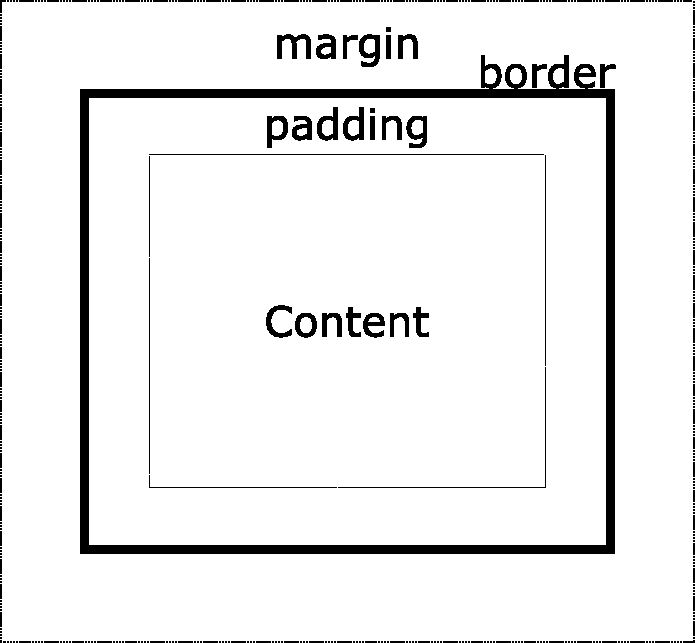
\includegraphics[keepaspectratio,width=\linewidth,height=\thirdh]
{diagrams/box-model.pdf}
\caption[CSS Box Model]{
The CSS box model defines the properties of boxes which wrap around HTML elements.
\imgcredit{Image drawn by the author of this thesis.}
}
\label{fig:BoxModel}
\end{figure}

In early versions of CSS, before the introduction of the Flexible Box
(Flexbox) layout module \parencite{CSSFlexboxFirstDraft}, the box
model was the only way to lay out elements. Style sheet authors had to
meticulously define margins of elements and their relative (or
absolute) positions in the document tree. The responsive capabilities
of this kind of layouting were very limited, because different
configurations for varying screen sizes had to be specified manually
using media queries. More complex features, like the filling of
available space, required manual implementation via scripting.





\subsection{CSS Flexbox Layout}
\label{sec:Flexbox}

CSS Flexible Box layout (Flexbox) \parencite{CSSFlexbox} is a
mechanism for one-dimensional layout of elements in either rows or
columns. This one-dimensionality is what separates it from grid-based
layout, which is inherently two-dimensional.
%
Even though the first draft of the Flexbox layout module was already
published in 2009 \parencite{CSSFlexboxFirstDraft}, implementations by
browser vendors have been a slow and bug-ridden process
\parencite{CanIUseCSSFlexbox}, which held back adoption by users for
several years after its inception. More recently though, partly
through the deprecation of Internet Explorer
\parencite{IEDeprecation}, all major browsers have mature
implementations of current Flexbox standards \parencite{CSSFlexbox},
and, in most cases, fallback styling is no longer necessary.

Flexbox layouting is enabled for child elements by setting the CSS
\cssname{display} property to \code{flex} on a container element. The
direction of the layout can then be specified using the CSS
\cssname{flex-direction} property which can be set to either
\code{row} or \code{column}.
%
The items inside a Flexbox container can have either a fixed or a
relative size. When items should be sized relative to the size of
their containers, the proportions of how the available space should be
divided can be controlled using ratios. These ratios can be set on
item elements via the CSS \cssname{flex} property.

Another important feature of Flexbox layout is the controllable
spacing of items, which can be specified separately for both the main
axis and the cross axis of the layout. Spacing along the main axis can
be configured with the CSS \cssname{justify-content} property, which
can take a number of different values and is illustrated in
Figure~\ref{fig:FlexboxJustifyContent}. Alignment of items on the
cross axis is achieved either by the CSS \cssname{align-items}
property on the container element or the CSS \cssname{align-self}
property on the items themselves.

\begin{figure}[tp]
\centering
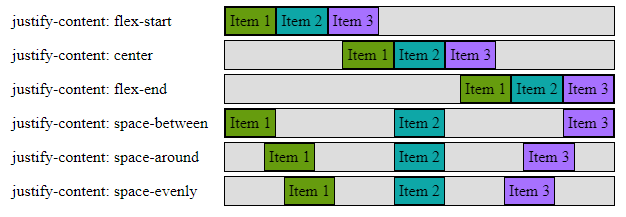
\includegraphics[keepaspectratio,width=\linewidth,height=\thirdh]
{images/flexbox-justify-content.png}
\caption[Flexbox CSS \cssname{justify-content} Property]{
The CSS \cssname{justify-content} property is used to distribute
items along the main axis of a Flexbox container. 
\imgcredit{Image created by the author of this thesis.}
}
\label{fig:FlexboxJustifyContent}
\end{figure}


This section only grazed the surface of what is possible with the
Flexbox layout module. There are many more useful CSS properties like
\cssname{flex-grow}, \cssname{flex-shrink}, and \cssname{flex-wrap}.
For a more detailed look at this topic it is recommended to review the
specification \parencite{CSSFlexbox} and read the excellent tutorial
by Chris Coyier \parencite{Coyier-FlexboxGuide}.





\subsection{CSS Grid Layout}
\label{sec:Grid}

The CSS Grid Layout Module \parencite{CSSGrid} defines the layout of
elements in a two-dimensional grid. The initial proposal of the CSS
Grid layout module was published in 2011 \parencite{CSSGridFirstDraft}
and has been further refined over the years. At the time of writing,
even though it still exists as merely a candidate recommendation for
standardization \parencite{CSSGrid}, many browsers have already
adopted it. Similar to the adoption of Flexbox, the history of browser
adoption of CSS Grid was initially strewn with inconsistencies and
bugs. However, in 2017 the major browsers Chrome, Firefox, Safari, and
Edge removed the need for vendor prefixes and implementations are now
considered stable \parencite{CanIUseCSSGrid}.

Grid layout of elements is enabled by setting the CSS
\cssname{display} property to \code{grid} on their container. The grid
in which items shall be laid out is then defined using the CSS
\cssname{grid-template-rows} and \cssname{grid-template-columns}
properties. In addition, the CSS \cssname{grid-template} property can
be used as a shorthand to simultaneously specify both the rows and
columns of a grid.
%
Item elements need to specify the cell of the grid into which they
shall be positioned. This is done with the CSS \cssname{grid-row} and
\cssname{grid-column} properties, which take the corresponding row and
column indices as values. Items can also be configured to span
multiple cells by specifying index ranges as the values of those
properties.

Every cell in a grid can also be assigned a specific name via the CSS
\cssname{grid-template-areas} property on the grid container element.
The items within the grid can then position themselves in specifically
named grid cells using the CSS \cssname{grid-area} property instead of
directly setting the row and column indices. The benefit of
positioning items this way is that the structure of the grid can be
freely changed without having to respecify the cells in which items
belong. As long as the new layout still specifies the same names of
cells somewhere in the grid, the items will be automatically placed at
their new positions.

There are also properties which control the layout of items within
grid cells and the layout of grid cells themselves. Similar to
Flexbox, this can be configured with the CSS \cssname{align-items} and
\cssname{justify-items} properties for laying out within grid cells,
and the CSS \cssname{align-content} and \cssname{justify-content}
properties for laying out the grid cells themselves. The latter
\cssname{*-content} properties only make sense when the cells do not
cover the full area of the grid. For a visual comparison between the
\cssname{*-items} and \cssname{*-content} properties, see
Figure~\ref{fig:GridLayoutProperties}.


\begin{figure}[tp]
\centering
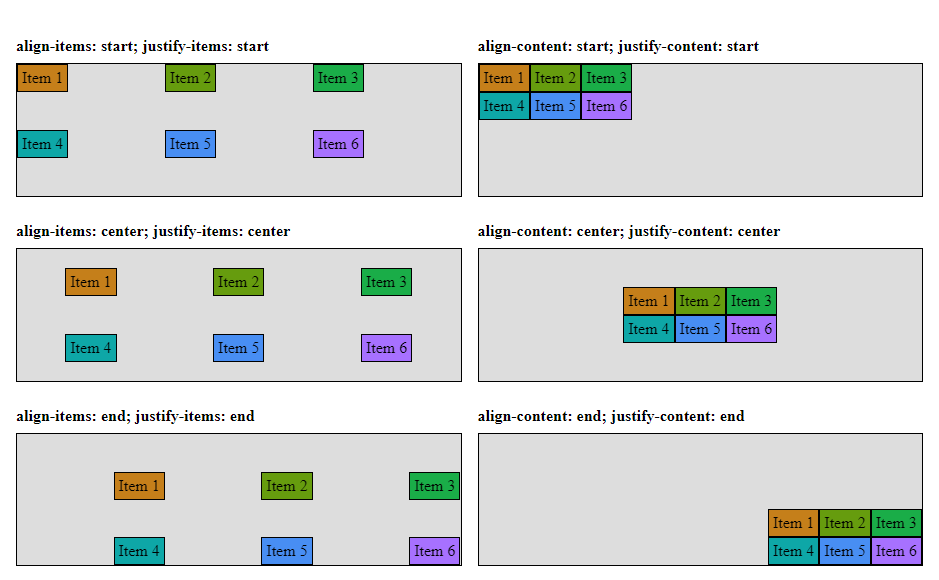
\includegraphics[keepaspectratio,width=\linewidth,height=\halfh]
{images/grid-layout-properties.png}
\caption[Grid Layout Property Comparision]{
The \cssname{*-items} properties are used to lay out items within
their grid cells, whereas the \cssname{*-content} properties are
used to lay out the grid cells themselves. 
\imgcredit{Image created by the author of this thesis.}
}
\label{fig:GridLayoutProperties}
\end{figure}


There is some apparent overlap between the CSS Grid and Flexbox layout
modules. At first sight, it seems like Grid layout supersedes Flexbox
layout, because everything which can be done using Flexbox layout can
also be done with Grid layout. While that is true, the inherent
difference in dimensionality and the resulting syntactic
characteristics lead to better suitability of one technology over the
other, depending on the context of use. As a general rule
\parencite{CSSGridVsFlexbox}, top-level layouts which require
two-dimensional positioning of elements are usually best implemented
using a Grid layout, whereas low-level layouts which merely need
laying out on a one-dimensional axis are better implemented using a
Flexbox layout.

For more details, the CSS Grid specification \parencite{CSSGrid} and
other sources like \textcite{GridLayoutInCSS} and
\textcite{House-GridGuide} are recommended.




\section{JavaScript (JS)}
\label{sec:JS}

JavaScript was originally developed as a client-side scripting
language run by an interpreter (engine) inside the web browser.
Nowadays, there are also standalone JavaScript engines and
environments like NodeJS \parencite{NodeJS}. JavaScript is a
multi-paradigm language which supports event-driven, as well as
functional and imperative programming. Driven by the popularity of the
web, JavaScript is currently the most used programming language
worldwide \parencite{StatisticProgrammingLanguageUsage}.

JavaScript was initially created by Netscape in 1995
\parencite{JSFirstRelease}. Before that, websites were only able to
display static content, which drastically limited the usefulness of
the web. Microsoft seemingly saw JavaScript as a potentially
revolutionary development, because they reverse-engineered Netscape's
implementation and published their own version of the language for
Internet Explorer in 1996 \parencite{JSIERelease}. The two
implementations were noticeably different from one another and the
uncontested monopoly of the Internet Explorer
\parencite{BrowserMarketShareEarly} held back standardization efforts
undertaken by Netscape \parencite{ECMAScript1}. When Firefox was
released in 2004 \parencite{FirefoxFirstRelease} and Chrome in 2008
\parencite{ChromeFirstRelease}, they quickly gained a considerable
share of the market \parencite{BrowserMarketShare}, as shown in
Figure~\ref{fig:BrowserMarketShare}. Galvanized by this new market
reality, all major browser vendors collaborated on the standardization
of JavaScript as ECMAScript 5 in 2009 \parencite{ECMAScript5}. Since
then, JavaScript has been continuously developed and its later
versions ECMAScript 2015 to 2021
\parencite{ECMAScript6, ECMAScript7, ECMAScript8, ECMAScript9, ECMAScript10, ECMAScript11, ECMAScript12}
are widely supported.


\begin{figure}[tp]
\centering
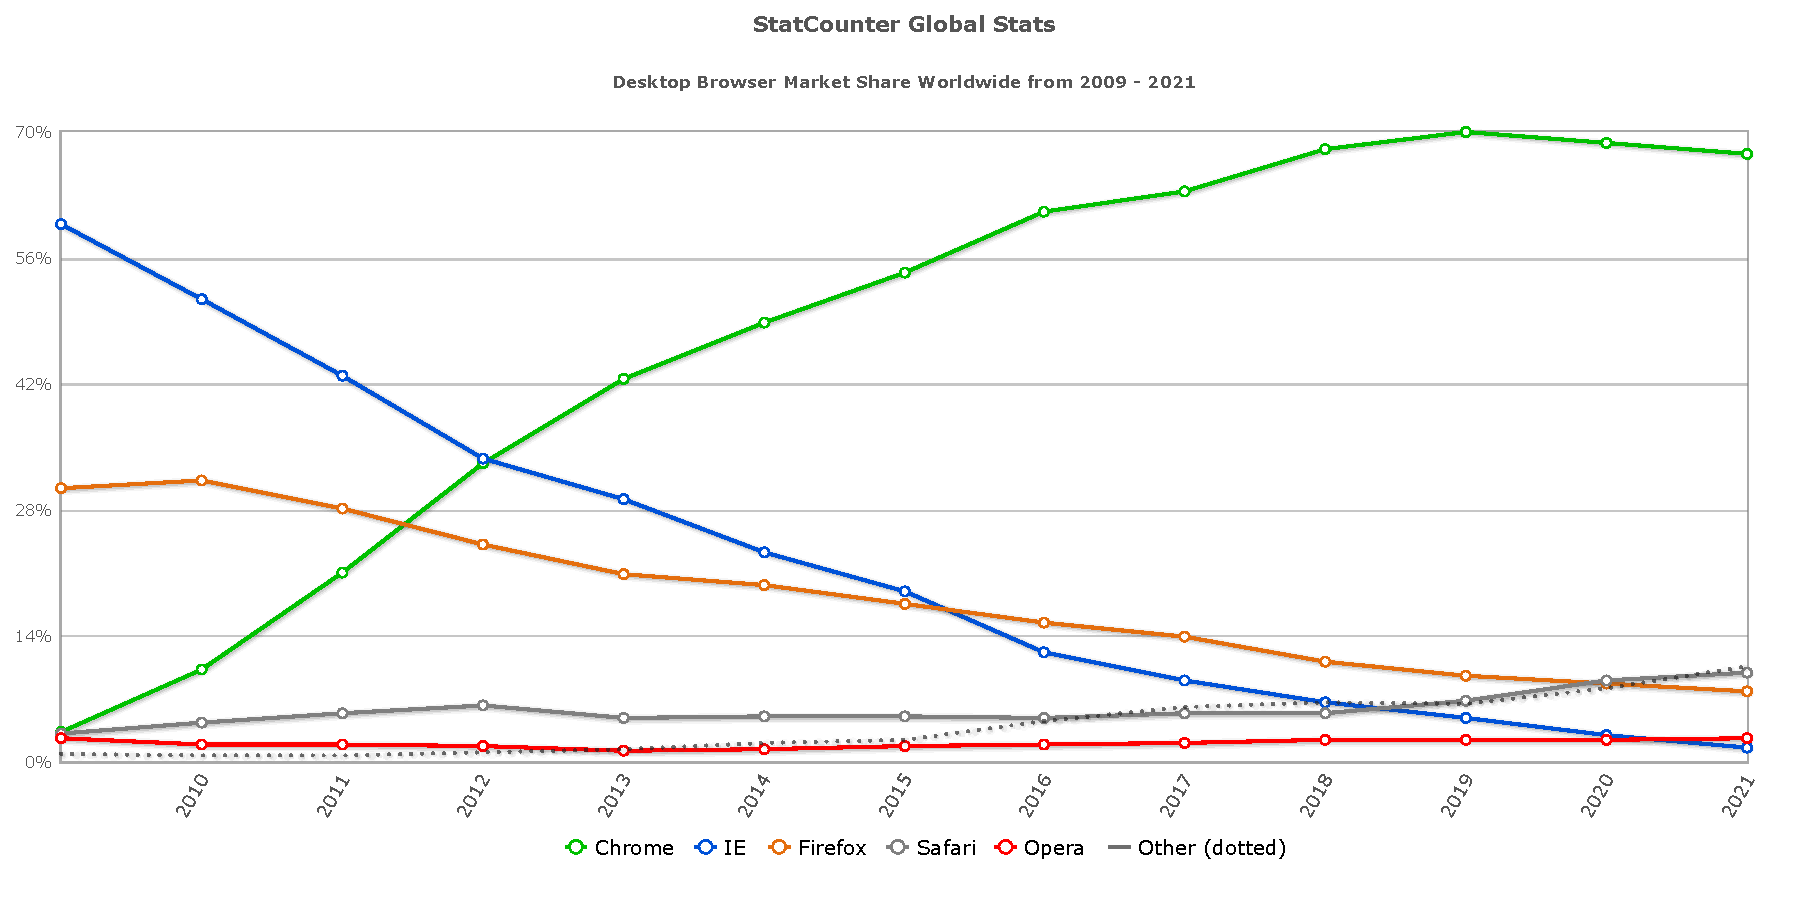
\includegraphics[keepaspectratio,width=\linewidth,height=\fullh / 3]{diagrams/browser-market-share.pdf}
\caption[Desktop Browser Market Share]{
  Since their release, Firefox and Chrome have contested the monopoly of the Internet Explorer and continuously gained more market share. 
  Recently, Chrome seems to be gaining an increasingly strong position within the market. 
  \imgcredit{Image taken from \textcite{BrowserMarketShare}}}
\label{fig:BrowserMarketShare}
\end{figure}


RespVis is a browser-based library which is designed to run within the
JavaScript engine of a browser. It builds heavily on widely supported
Web APIs, which are JavaScript modules specifically meant for
development of web pages. These Web APIs are standardized by the W3C
and each browser has to individually implement them in their
JavaScript engine.

The most popular Web API, which every web developer is familiar with,
is the Document Object Model (DOM). The DOM is the programming
interface and data representation of a web page or document.
Internally, a document is modeled as a tree of objects, where each
object corresponds to a specific HTML or SVG element in the document
hierarchy and its associated data and functions. In addition to the
querying of elements, the DOM also defines functionality to mutate
them and their attributes, as well as functionality for handling and
dispatching events. It also exposes the mechanism of
\modname{MutationObservers}, which are used to observe changes of
attributes and children in the document tree. The initial
specification of the DOM was published in 1997 \parencite{DOM1}. It
is currently maintained as a living standard by the WHATWG
\parencite{DOM}.

Another important Web API in the context of this work is the
\modname{ResizeObserver} API. It provides the ability to observe an
element's size and respond to changes, which increases the responsive
capabilities of websites. Previously, scripts could only respond to
changes in the overall viewport size via the \code{resize} event
on the \code{window} object, but this meant that changes of an
individual element's size through attribute changes could not be
detected. This limitation is fixed with the \modname{ResizeObserver}
API, which is already fully supported by all modern browsers, even
though it has so far only been published as an editor's draft
\parencite{ResizeObserver}.






\section{TypeScript (TS)}
\label{sec:TS}

TypeScript (TS) is a strongly-typed programming language which is
designed as an extension of JavaScript. Syntactically, it is a
superset of JavaScript which enables the annotation of properties,
variables, parameters, and return values with types. It requires a
transpiler (compiler) to convert the TypeScript code into valid
JavaScript code for a specific ECMAScript version.

Initially, TypeScript was released by Microsoft in 2012
\parencite{TSFirstRelease} to extend JavaScript with features which
were already present in more mature languages, and whose absence in
JavaScript caused difficulties when working on larger codebases. At
the time of TypeScript's initial development, it provided features
which would later be offered by ECMAScript 6, including a module
system to be able to split source code into reusable chunks and a
class system to aid object-oriented development. TypeScript code using
these features could then be transpiled into standard-conformant
JavaScript code, which could be interpreted by JavaScript engines of
the time. At the time of writing, ECMAScript 6 is widely supported by
all modern browsers and therefore the main benefit of TypeScript over
JavaScript lies in its provision of a static type system.

The extension of JavaScript with a static type system brings many
benefits, including the improved tooling which comes with
type-annotated code. Tools such as linters \parencite{ESLint} are able
to point out errors early in development and assist developers with
automated fixes, improved code completion, and code navigation.
Additionally, studies like \textcite{ToTypeOrNotToType} looked at
software bugs in publicly available codebases and found that 15\% of
them could have been prevented with static type checking.

The TypeScript type system was designed to support JavaScript
constructs as completely as possible, via structural types and unified
object types. Another goal was to make the type annotation of
JavaScript code as effortless as possible to improve adoption by
existing projects. This was done by consciously allowing the type
system to be statically unsound via gradual typing and also by
employing type inference to reduce the number of necessary
annotations. The major properties of TypeScript's type system design
are summarized in Table~\ref{tab:TSTypeSystemDesignProperties}.


\begin{table}[tp]
\tablestretch
\rowcolors{2}{}{tablerowcolour}
\centering
\begin{tabularx}{\linewidth}{>{\kern-\tabcolsep}lX<{\kern-\tabcolsep}}
\toprule
Design Property & Description \\
\midrule
Full erasure         &
Types are completely removed by the compiler, there is no type checking at runtime. \\
%
Type inference       &
Many types can be inferred from usage, minimizing the number of types which have to be explicitly stated. \\
%
Gradual typing       &
Type checking can be selectively prevented using the dynamic type \lstinline{any}. \\
%
Structural types     &
Types are defined via their structure as opposed to via their names.
This better fits JavaScript, where objects are usually custom-built and used based on their shapes. \\
%
Unified object types &
A type can simultaneously describe objects, functions, and arrays.
These constructs are common in JavaScript and thus TypeScript needs to support their typing. \\
\bottomrule
\end{tabularx}
\caption[TypeScript Type System Design Properties]{
A summary of the major design properties on which TypeScript's type system is built.
\imgcredit{Table created by the author of this thesis with data from \textcite{UnderstandingTS}.}
}
\label{tab:TSTypeSystemDesignProperties}
\end{table}









\section{Web Graphics}
\label{sec:WebGraphics}

Graphics are used as a medium for visual expression to enhance the
representation of information on the web. There are many fields of
application like the integration of maps, photographs, or charts in a
web page. Multiple complementary technologies exist for web graphics,
each with particular strengths and weaknesses depending on the use
case. These technologies include pixel-based raster images, Scalable
Vector Graphics (SVG), and 2d and 3d graphics through the
\elname{<canvas>} element.



\subsection{Raster Images}
\label{sec:RasterImages}

A raster image represents a graphic as a rectangular, two-dimensional
grid of pixels with a fixed size (resolution) in each dimension.
Whenever a raster image is scaled up or down to a different size,
visual artifacts become very apparent, as can be seen in
Figure~\ref{fig:RasterImage}. Raster images are either created by
image capturing devices or special editing software and saved as
binary files in varying formats. The most widely used formats for
raster images are JPEG \parencite{JPEG} and PNG (Portable Network
Graphics) \parencite{PNG}. JPEG has lossy compression, which achieves
low file sizes whilst retaining reasonable image quality, and is
typically used for photographs. PNG has lossless compression, which
compresses well whilst preserving every original pixel as is, and also
supports transparency. Both formats support progressive rendering as
an image is loaded.


\begin{figure}[tp]
\centering
\subfloat[Intended size.]{%
\hspace{1cm}

\includegraphics[scale=1]{images/circle.png}
\hspace{1cm}
\label{fig:RasterImage1}
}
\hspace{1cm}
\subfloat[Two and a half times intended size.]{%
\hspace{1cm}

\includegraphics[scale=2.5]{images/circle.png}
\hspace{1cm}
\label{fig:RasterImage2}
}
\caption[Raster Image Scaling]{%
A raster image of a circle.
Pixelation artifacts become very apparent when a raster image
is scaled to a different size.
\imgcredit{Image created by the author of this thesis.}
}
\label{fig:RasterImage}
\end{figure}


Raster images are embedded into documents in binary format. This means
that the contents of the graphic are not accessible in a non-visual
representation. To make the information accessible to visually
impaired people, an additional textual description of the graphic's
content must be provided via the \attrname{alt} and
\attrname{longdesc} attributes.





\subsection{Scalable Vector Graphics (SVG)}
\label{sec:SVG}

Vector graphics describe an image in terms of objects and shapes, such
as lines, circles, polygons, and text. They can be scaled freely
without loss of quality. Scalable Vector Graphics (SVG) is an
XML-based format for vector graphics. It was initially published by
the W3C in 1999 \parencite{SVG1}, SVG 1.1 \parencite{SVG11} is the
latest version that is widely supported by browsers, and support for
SVG 2 \parencite{SVG2} is currently on its way. Graphics in an SVG
file can be specified in a normalised coordinate space (inside a
viewBox), enabling them to be freely scaled. Since SVG files are XML,
they can be created with any text editor, but numerous tools and
editors such as Inkscape \parencite{Inkscape} and Illustrator
\parencite{Illustrator} exist to create or export SVG. A simple example
of an SVG document containing a single circle can be seen in
Listing~\ref{list:SVG}, with its visualization shown in
Figure~\ref{fig:SVG}.

\begin{samepage}
\lstinputlisting[%
  float=tp,
  aboveskip=\floatsep,
  belowskip=\floatsep,
  xleftmargin=0cm,              % no extra margins for floats
  xrightmargin=0cm,             % no extra margins for floats
  basicstyle=\footnotesize\ttfamily,
  frame=shadowbox,
  numbers=left,
  label=list:SVG,
  caption={%
[SVG Document Containing a Circle]%
A simple SVG document containing a \elname{<circle>} element.
The visual representation of this document in different sizes
is shown in Figure~\ref{fig:SVG}.
}
]{listings/circle.svg}
\end{samepage}


\begin{figure}[tp]
\centering
\subfloat[Intended size.]{%
\hspace{1cm}

\includegraphics[scale=1]{images/circle.pdf}
\hspace{1cm}
\label{fig:SVG1}
}
\hspace{1cm}
\subfloat[Two and a half times intended size.]{%
\hspace{1cm}

\includegraphics[scale=2.5]{images/circle.pdf}
\hspace{1cm}
\label{fig:SVG2}
}
\caption[SVG Scaling]{%
SVG documents can be scaled freely without pixelation artifacts.
Here, the SVG document from Listing~\ref{list:SVG} is shown.
\imgcredit{Image created by the author of this thesis.}
}
\label{fig:SVG}
\end{figure}



The encoding in XML leads to SVG being the best format to represent
graphics in terms of accessibility. Graphics are directly saved in a
hierarchical and textual form which describes their shapes and how
they are composed. In addition to the shapes being inherently
accessible, the various elements of an SVG document can be annotated
with further information to aid comprehension when consumed in a
non-visual way.

SVG files are XML documents whose meta format is described in a
special SVG namespace. Web browsers support mixing of HTML and SVG
elements in a web page, and the SVG elements can be accessed by
scripts via the DOM Web API just like HTML elements.

The most widely supported way of styling SVG elements is via
attributes, which is supported by every software dealing with SVG
files. However, the specification aims for maximum compatibility with
HTML, and therefore it is also possible to use CSS to style and
animate SVG elements when they are rendered in a browser. Using CSS to
separate presentation from content has many benefits, which were
already described in Section~\ref{sec:CSS}. Unfortunately, it is not
possible to style every SVG attribute with CSS, only so-called
presentation attributes like \attrname{fill} and \attrname{stroke-width}
are available through CSS. These presentation attributes are listed in
the SVG specification \parencite{SVG11} and will be extended by
additional attributes like \cssname{x}, \cssname{y}, \cssname{width}
and \cssname{height} in upcoming releases \parencite{SVG2}.


\subsection{Canvas (2D)}
\label{sec:Canvas2D}

The \elname{<canvas>} element was introduced in HTML5
\parencite{HTML5} and is used to define a two-dimensional, rectangular
region in a document which can be drawn into by scripts. Even though
rendering of dynamic graphics as \elname{<canvas>} elements is often
faster than representing them as SVG documents, their use is
explicitly discouraged by the WHATWG \parencite{HTML} when another
suitable representation is possible. The reasons for this are that
\elname{<canvas>} elements are not compatible with other web
technologies like CSS or the DOM Web API and because the resulting
rendering provides only very limited possibilities for accessibility.

The graphics are drawn via a low-level API provided by the rendering
context of a particular canvas. The two most significant rendering
contexts are \code{2d} and \code{webgl}.

The \code{2d} rendering context enables platform-independent 2d
rendering via a software renderer, whose API is standardized directly
in the canvas specification \parencite{Canvas2D}. An example of an
HTML document containing two differently sized canvases into which
responsive circles are drawn using a 2d rendering context can be seen
in Listing~\ref{list:Canvas} with the corresponding visual output in
Figure~\ref{fig:Canvas}.


\begin{samepage}
\lstinputlisting[%
  float=tp,
  aboveskip=\floatsep,
  belowskip=\floatsep,
  xleftmargin=0cm,              % no extra margins for floats
  xrightmargin=0cm,             % no extra margins for floats
  basicstyle=\footnotesize\ttfamily,
  frame=shadowbox,
  numbers=left,
  label=list:Canvas,
  caption={%
[Canvas With Responsive Circles]%
A basic HTML document containing two canvases of different sizes
which render circles relative to the canvas size. 
The visual representation of this document is shown in Figure~\ref{fig:Canvas}.
}
]{listings/canvas.html}
\end{samepage}


\begin{figure}[tp]
\centering
\subfloat[100-pixel canvas.]{%
\hspace{1cm}

\includegraphics[scale=0.5]{images/canvas100.png}
\hspace{1cm}
\label{fig:Canvas1}
}
\hspace{1cm}
\subfloat[250-pixel canvas.]{%
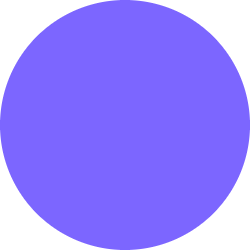
\includegraphics[scale=0.5]{images/canvas250.png}
\label{fig:Canvas2}
}
\caption[Canvas With Responsive Circles]{
Responsive rendering of graphics inside \elname{<canvas>} elements has to be
implemented manually by calculating everything relative to its dimensions. 
This figure shows the visual output
of the canvas example in Listing~\ref{list:Canvas}. 
\imgcredit{Image created by the author of this thesis.}
}
\label{fig:Canvas}
\end{figure}







\subsection{Canvas (WebGL)}
\label{sec:CanvasWebGL}

The \code{webgl} rendering context enables 3d drawing through the
WebGL version 1 API \parencite{WebGL1}. The \code{webgl2}
rendering context enables 3d drawing through the WebGL version 2 API
\parencite{WebGL2}. WebGL-based rendering is hardware-accelerated and
often much faster than rendering via a 2d canvas or SVG. It is also
possible to render 2d graphics using a WebGL render context, but the
necessary setup and rendering API is rather complex.   



\section{Layout Engines}
\label{sec:LayoutEngines}

A layout engine is used to calculate the boundary coordinates of
visual components based on input components annotated with layout
constraints. These layout constraints describe the size and position
of components and their relationships between each other in a syntax
understood by the layout engine. For browser-based layout engines, the
input components are normally declared as HTML documents, which are
constrained using CSS. More low-level layout engines require custom
formats, which usually involve a hierarchy of objects constrained
using specific properties. The most relevant layout engines in the
context of this work are summarized in the following sections.


\subsection{Browser Engines}
\label{sec:BrowserEngines}

The purpose of a browser engine is to transform document and any
additional resources, like CSS, into a visual representation. A
browser engine is a core component of every web browser, and it is
responsible for laying out elements and rendering them.  The
terminology of browser engines is ill-defined, with them sometimes
also being referred to as layout or render engines. Theoretically, the
layout and render processes could be separated into different
components, but in practice they are tightly-coupled into a combined
component, which will be referred to as a browser engine in this work.
Some notable browser engines are WebKit \parencite{WebKit}, Blink
\parencite{Blink}, and Gecko \parencite{Gecko}.

In a browser engine, the layout of elements is constrained with CSS,
which yields great flexibility as already described in
Section~\ref{sec:CSS}. A range of mechanisms is available to precisely
control the layout of elements, like the Flexible Box and Grid layout
modules, which can also be used in combination.

The layout module of a browser engine can only be invoked directly by
browsers to position HTML elements in actively rendered documents. To
use it for calculating layouts of non-HTML constructs, they must be
replicated in active documents, so they can be parsed, laid out and
rendered by the browser engine. These replicated constructs do not
necessarily have to be visible, and they could also be removed from
the document after the layout has been acquired, meaning they do not
need to be noticeable at all. A strong limitation of using browser
engines to calculate layouts is that it requires a browser runtime to
work and, even though there are solutions like Electron
\parencite{Electron} available, which enable development of desktop
applications using web technologies, this limitation forces
applications into a very specific stack of technologies.



\subsection{Yoga}
\label{sec:Yoga}

Yoga \parencite{Yoga} is a layout engine which enables the computation
of layouts constrained using the grammar defined in the CSS Flexible
Box layout module (see Section~\ref{sec:Flexbox}). It has been
maintained by Facebook as an open-source project since 2016
\parencite{YogaRelease}, with the goal of providing a small and
high-performance library which can be used across all platforms. Yoga
is implemented in C/C++, which works on a myriad of devices, with
bindings available for other platforms like JavaScript, Android, and
iOS. It has been widely adopted and is used to perform layouting in
major frameworks such as React Native \parencite{ReactNative}, Litho
\parencite{Litho}, and ComponentKit \parencite{ComponentKit}.



\subsection{FaberJS}
\label{sec:FaberJS}

FaberJS \parencite{FaberJS} is a layout engine very similar to the
Yoga layout engine in that it enables the computation of layouts for
constructs other than HTML documents, using a layout grammar
originally created for CSS. In contrast to Yoga, which is used to
create one-dimensional layouts using the Flexbox layout grammar,
FaberJS implements a two-dimensional layout algorithm built on the
grammar of the CSS Grid layout module (see Section~\ref{sec:Grid}).
This inherently two-dimensional approach to layouting is more suited
to information visualization than a one-dimensional approach. FaberJS
is an open-source JavaScript project developed since 2019 by
Idera. Even though the layouts it computes are constrained with the
Grid Layout grammar, it only supports a subset the functionality
defined in the original CSS module. Some examples of missing
functionaly include missing support for margins, gaps, and the
\cssname{*-content} and \cssname{grid-auto-*} properties. Working
around the limitations caused by these missing features is
non-trivial, and it seems unlikely that support for them will be added
by the FaberJS maintainers in the near future because, at the time of
writing, the project has not been updated in nearly two years.






\section{Responsive Web Design}
\label{sec:RWD}

Influenced by the increasing use of mobile devices and their vastly
varying screen sizes, responsive web design has established itself as
the predominant way of designing web pages. The core idea of
responsive web design is that instead of designing pages for different
types of devices, website authors create a single design for a page,
which adapts to the characteristics of the consuming device. The term
\enquote{Responsive Web Design} was initially defined by
\textcite{Marcotte-ALA-RWD} and later compiled into a book
\parencite{ResponsiveWebDesign}, in which the author differentiates
between flexible and responsive web designs. A flexible web design,
which merely fluidly scales blocks of content to make them fit into
the width of a browser window, is not enough to provide a good
experience for users. Such designs will work well enough for similarly
sized viewports to the one they were created for, but they will lead
to noticeable artifacts on lower resolutions.

These problems can be avoided by positioning the individual components
of a page in a manner which provides them with enough space to render
correctly. This can be achieved by using CSS media queries to adapt
the overall layout of a page to the dimensions of the consuming
device. Another crucial part of responsive web design is to support
the different modes of interaction inherent to the various types of
devices used to access the web. Desktop users might access a website
using a mouse, mobile device users typically interact via a
touchscreen, and yet others might consume a page in a purely textual
form with a screen reader and interact via a keyboard. It is one of
the mantras of responsive web design to provide smooth and complete
access to information to all users, regardless of the device they are
using.
          %   Chapter 2

\cleardoublepage
\chapter{Information Visualization}
\label{chap:InfoVis}

Information visualization is the science of representing abstract information as interactive graphics to present and analyze it more efficiently. 
These two goals of presenting and analyzing abstract information in a visual form are built on the properties of human visual perception, which include the rapid scanning, recognition and recollection of visual information as well as the automatic detection of patterns in it.
In contrast to textual representations of data, the processing of well-designed visualizations requires much less cognitive effort because it leverages features of the human visual processing system such as preattentive processing, meaning that certain visual attributes can be processed very quickly and without any conscious effort \parencite{PreattentiveProcessing}. 

In addition to visuals being easier to assimilate by humans, a purely textual and statistical view on data can also lead to erroneous assumptions as demonstrated by \cite{AnscombesQuartet} in the infamous visualization of four completely different datasets that have identical summary statistics, called Anscombe's Quartet. An observer trying to understand these sets of data purely from their statistics would mistakenly deem them to be identical because their inequality will only become obvious after carefully examining and comparing the individual entries in the datasets themselves, which is a tedious and error-prone task when not aided by visual representations like Figure \ref{fig:AnscombesQuartet}. Even though Anscombe's Quartet is very likely the most famous example to demonstrate this characteristic, it is certainly not the only set of datasets that possesses it, as has been shown by \cite{GenDataIdenticalStatisticsDissimilarGraphics}.

\begin{figure}[tp]
    \centering
    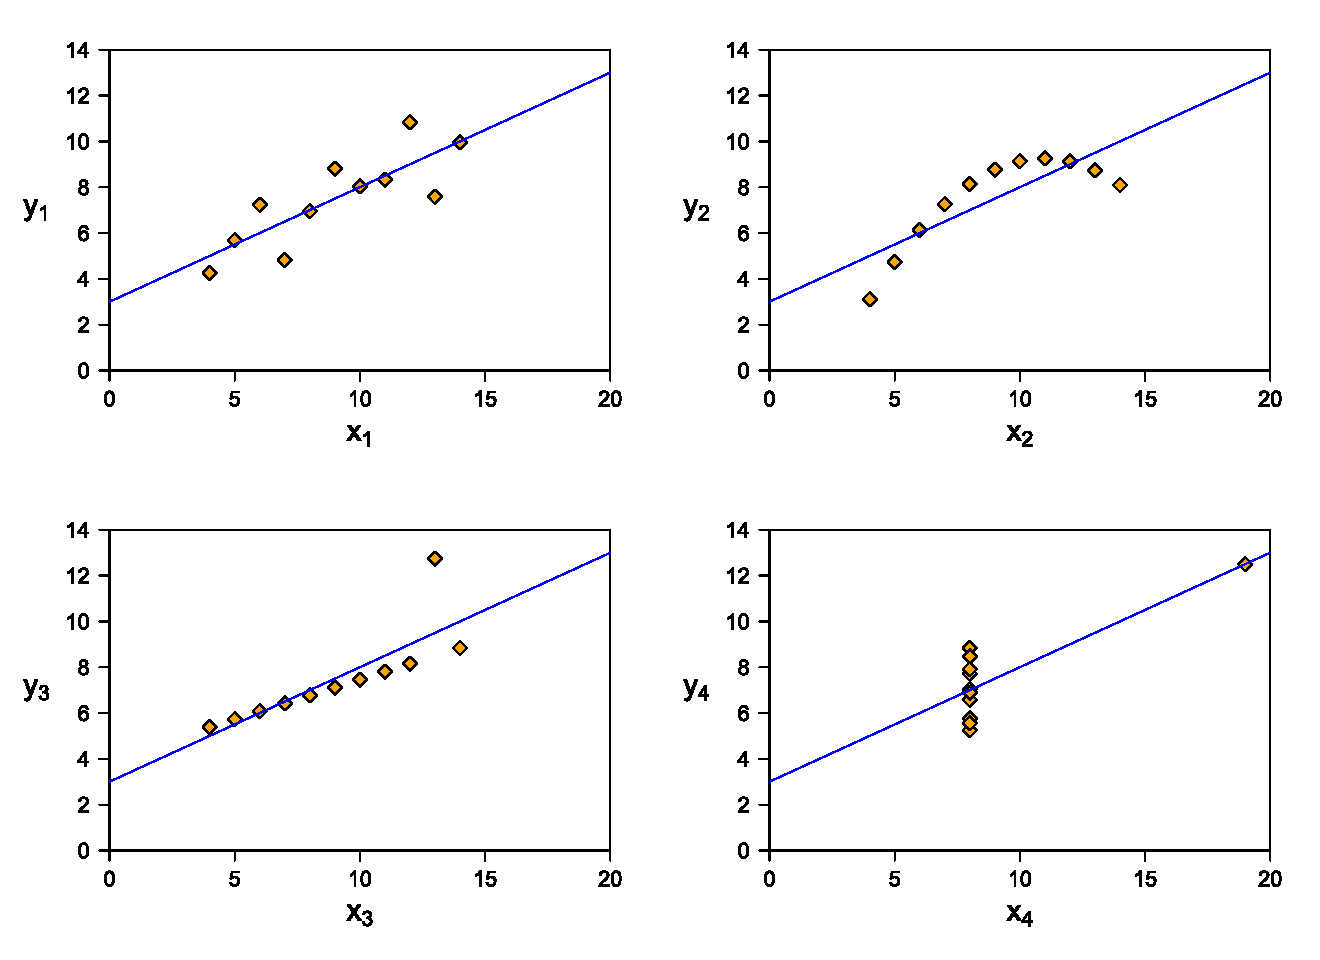
\includegraphics[keepaspectratio,width=\linewidth,height=\fullh / 3]
    {diagrams/anscombe.pdf}

    \caption[Anscombe's Quartet]{
        Anscombe's Quartet consists of four distinct sets of data that share identical summary statistics. The difference between these datasets is only obvious by carefully examining the textual data or by plotting it. \imgcredit{Image extracted from \cite{IVISCourseNotes}. Used with kind permission by Keith Andrews.}
    }
    \label{fig:AnscombesQuartet}
\end{figure}

Regarding terminology, this work adheres to the separation of the field of visualization into three main subfields as described by \cite{IVISCourseNotes}.

\begin{enumerate}
    \item Information Visualization: Deals with abstract data, which has no inherent presentation and for which a suitable type of visualization has to be chosen.
    \item Geographic Visualization: Deals with map-based data that has an inherent spatial dimension. 
    \item Scientific Visualization: Deals with object-related data that has inherent presentation, which is usually related to the object's real world representation.
\end{enumerate}

In addition to these three subfields, \cite{IVISCourseNotes} defines the often used term Data Visualization as the intersection of Geographic Visualization and Information Visualization. Therefore, it deals with visualizing spatial as well as abstract data.

Visualizations presented in an interactive medium do not merely consist of visual representations. In order to analyze more complex datasets, it is equally important to provide means for interacting with these representations because without interaction, a visualization becomes a static image, which has only very limited usefulness when dealing with large and multidimensional data. Even though the majority of the attention in the field of Information Visualization has been put on the presentational aspect of visualizations, a lot of research has also been conducted on their interactive aspects. Many taxonomies have been formulated with the goal of defining the design space of interactions to support analytic reasoning, but they vary greatly depending on the concepts they are focusing on. Some taxonomies have been defined on the concept of low-level interaction techniques \parencite{TheEyesHaveIt,GrammarOfGraphics}, providing a very system-centric view on interaction, while other taxonomies focus on user tasks \parencite{LowLevelComponentsOfAnalyticActivity} without them being tightly bound to interacting with visualizations. \cite{RoleOfInteractionInInformationVisualization} aims to provide a view that is in between the purely system-centric and purely user-centric extremes by defining a taxonomy based on user intent. The categories of this taxonomy are listed in Table \ref{tab:UserIntentCategories}, and they form a good framework with which interactivity in the context of Information Visualization can be discussed. 

\begin{table}[tp]
    \centering
    \begin{tabularx}{\linewidth}{| l | X | X |}
        \hline
        \textbf{Category} & \textbf{Description} & \textbf{Examples} \\ \hline
        Select & Mark items as interesting. &  \\ \hline
        Explore & Show different items. & Panning, direct-walk  \\ \hline
        Reconfigure & Show a different arrangement. & Dimension configuration, position adjustments \\ \hline
        Encode & Show a different representation. & Change chart type, orientation, colors, shapes, ... \\ \hline
        Abstract/Elaborate & Show more or less detail. & Details-on-demand (drill-down, sunburst, tooltips, zooming)  \\ \hline
        Filter & Show items based on conditions. & Dynamic query controls   \\ \hline
        Connect & Show related items. & Highlight connected items, highlight item in different representations   \\ \hline
        
    \end{tabularx}
    \caption[Categories of Interaction Based on User Intent]
    {
        This table shows the different categories of interacting with visualizations based on user intent.
        \imgcredit{Table adapted from \cite{RoleOfInteractionInInformationVisualization}}
    }
    \label{tab:UserIntentCategories}
\end{table}

\section{History of Information Visualization}

The history of Information Visualization goes back a long time with one of the earliest examples dating back to the 10th century, when an unknown astronomer created a chart about the movement of the most prominent planets \parencite{CommentariiInSomniumScipionis}, shown in Figure \ref{fig:PlanetaryMovements}. Other noteworthy early visualizations include the first occurrence of the principle \cite{VisualDisplayOfQuantitativeInformation} later coined "small multiples" in a 1626 chart demonstrating sunspot changes (Figure \ref{fig:SunspotChanges}) by \cite{RosaUrsina} and a 1644 chart displaying longitudinal distance determinations between Toledo and Rome (Figure \ref{fig:RomeToledoLongitude}) by Michael Florent van Langren. 

\begin{figure}[tp]
    \centering
    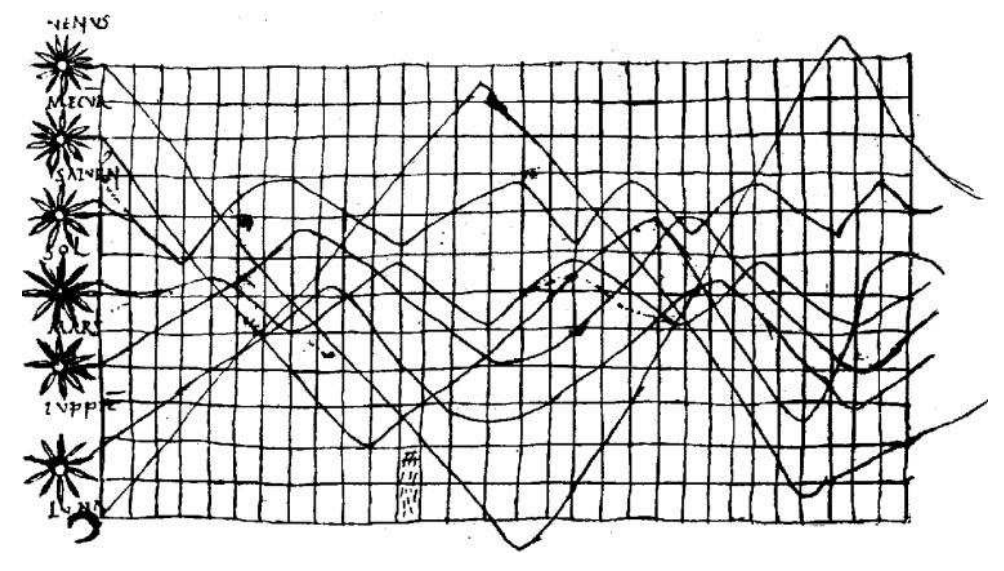
\includegraphics[keepaspectratio,width=\linewidth,height=\fullh / 3]
    {images/planetary-movements.png}
    \caption[Chart of Planetary Movements from the Tenth Century]{
        A chart created by an unknown astronomer in the tenth century depicting the movements of the seven most prominent planets. \imgcredit{Image extracted from \cite{BriefHistoryOfDataVis}. Original appearance in \cite{CommentariiInSomniumScipionis}.}
    }
    \label{fig:PlanetaryMovements}
\end{figure}

\begin{figure}[tp]
    \centering
    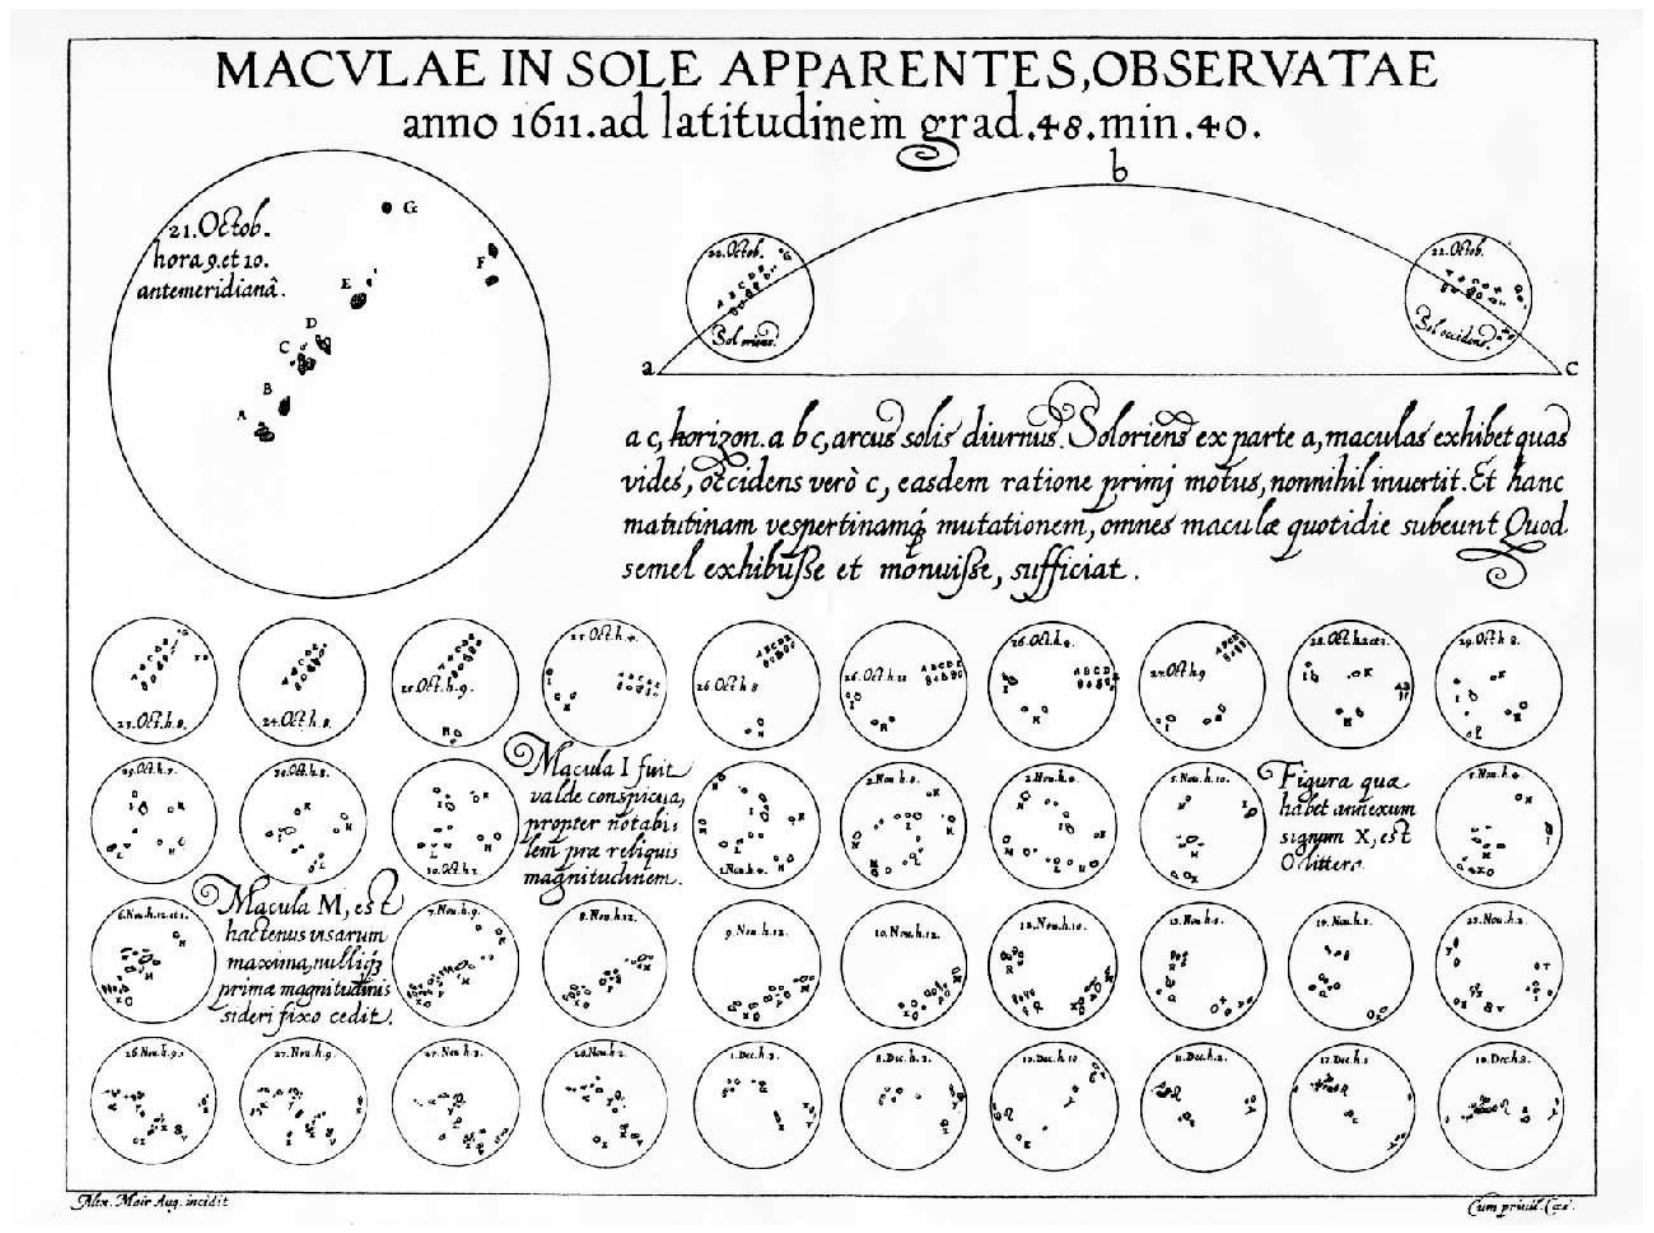
\includegraphics[keepaspectratio,width=\linewidth,height=\fullh / 3]
    {images/sunspot-changes.png}
    \caption[Chart of Changes in Sunspots from 1626]{
        This chart shows the observed changes in sunspots based on recordings of two months of data from 1611. It is the first occurrence of the principle later called "small multiples" by \cite{VisualDisplayOfQuantitativeInformation}. \imgcredit{Image extracted from \cite{BriefHistoryOfDataVis}. Original appearance in \cite{RosaUrsina}.}
    }
    \label{fig:SunspotChanges}
\end{figure}

\begin{figure}[tp]
    \centering
    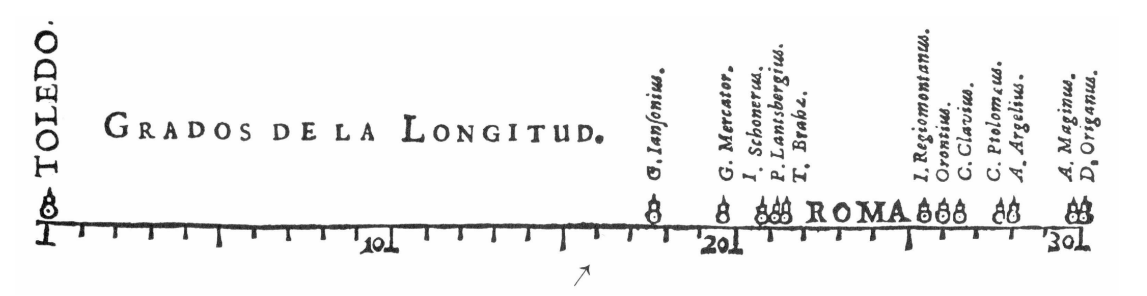
\includegraphics[keepaspectratio,width=\linewidth,height=\fullh / 3]
    {images/rome-toledo-longitude.png}
    \caption[Chart of Longitudinal Distance Determinations Between Toledo and Rome From 1644]{
        This chart compares the twelve known estimates in longitudinal distance between Rome and Toledo by various astronomers. The correct distance is marked by the arrow beneath. It is considered to be the first visual representation of statistical data. \imgcredit{Image extracted from \cite{BriefHistoryOfDataVis}. Original appearance in \cite{VisualExplanations}.}
    }
    \label{fig:RomeToledoLongitude}
\end{figure}

William Playfair (1759 - 1823) is by many considered to be one of the forefathers of modern visualizations because his published works contain the first occurrences of many graphical forms that are still widely used today. In one of his earlier works \parencite{CommercialAndPoliticalAtlas} he introduced the concepts of line (Figure \ref{fig:PlayfairLineChart}), bar (Figure \ref{fig:PlayfairBarChart}) and area charts (Figure \ref{fig:PlayfairAreaChart}) to communicate economic factors of England during the eighteenth century. In a related later work \parencite{StatisticalBreviary} he uses the first ever published pie and circle charts to show and compare the resources of states and kingdoms in Europe. The charts he created are very similar to modern ones because they already contain all the major elements found in today's visualizations, such as labeled axes, grids, titles and color-based categorization.

\begin{figure}[tp]
    \centering
    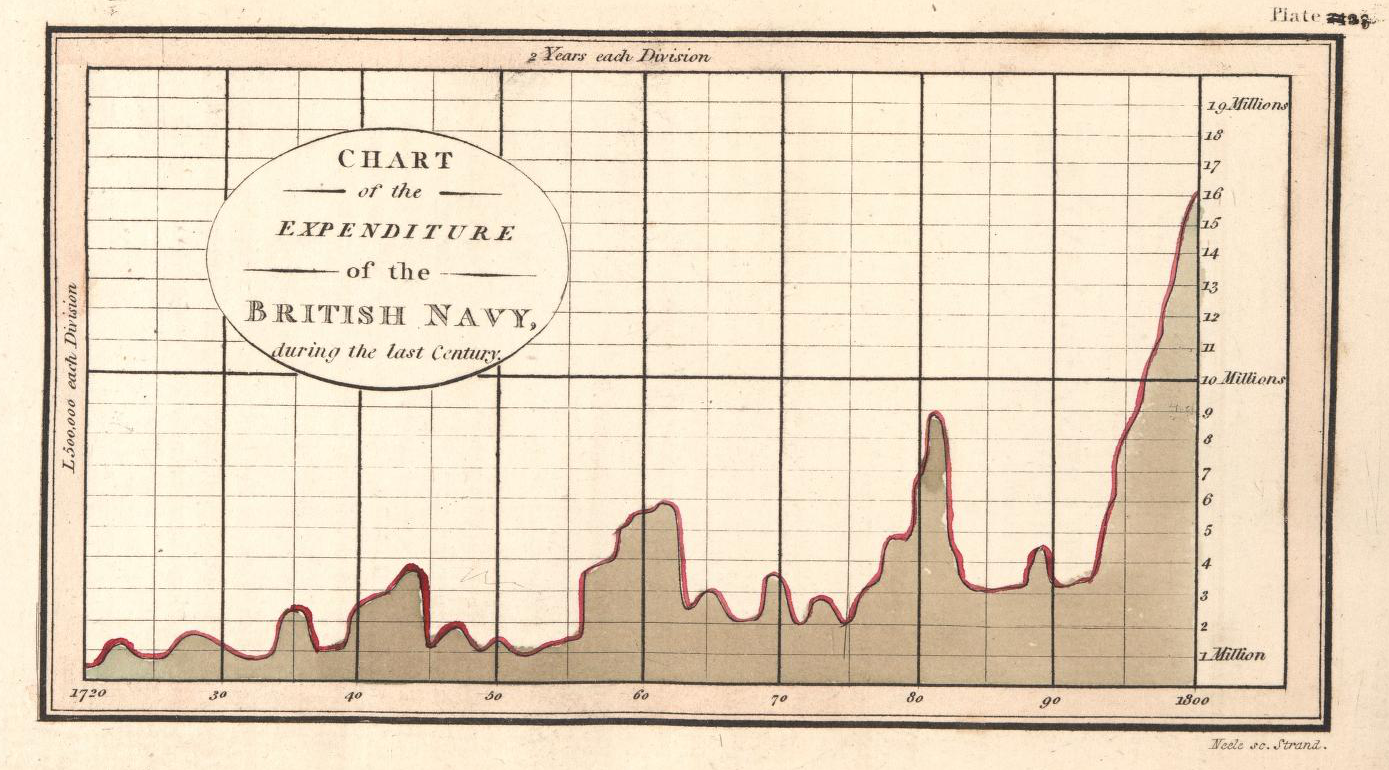
\includegraphics[keepaspectratio,width=\linewidth,height=\fullh / 3]
    {images/playfair-line-chart.png}
    \caption[Line Chart by William Playfair From 1786]{
        This chart shows the expenditure of the British navy during the eighteenth century as a line chart. It was published in 1786 and is considered to be one of the first occurrences of a line chart that contains all components found in modern visualizations. \imgcredit{Image extracted from Schoenberg Center for Electronic Text and Image (SCETI). Used under the terms of Creative Commons CC BY 2.5.}
    }
    \label{fig:PlayfairLineChart}
\end{figure}

\begin{figure}[tp]
    \centering
    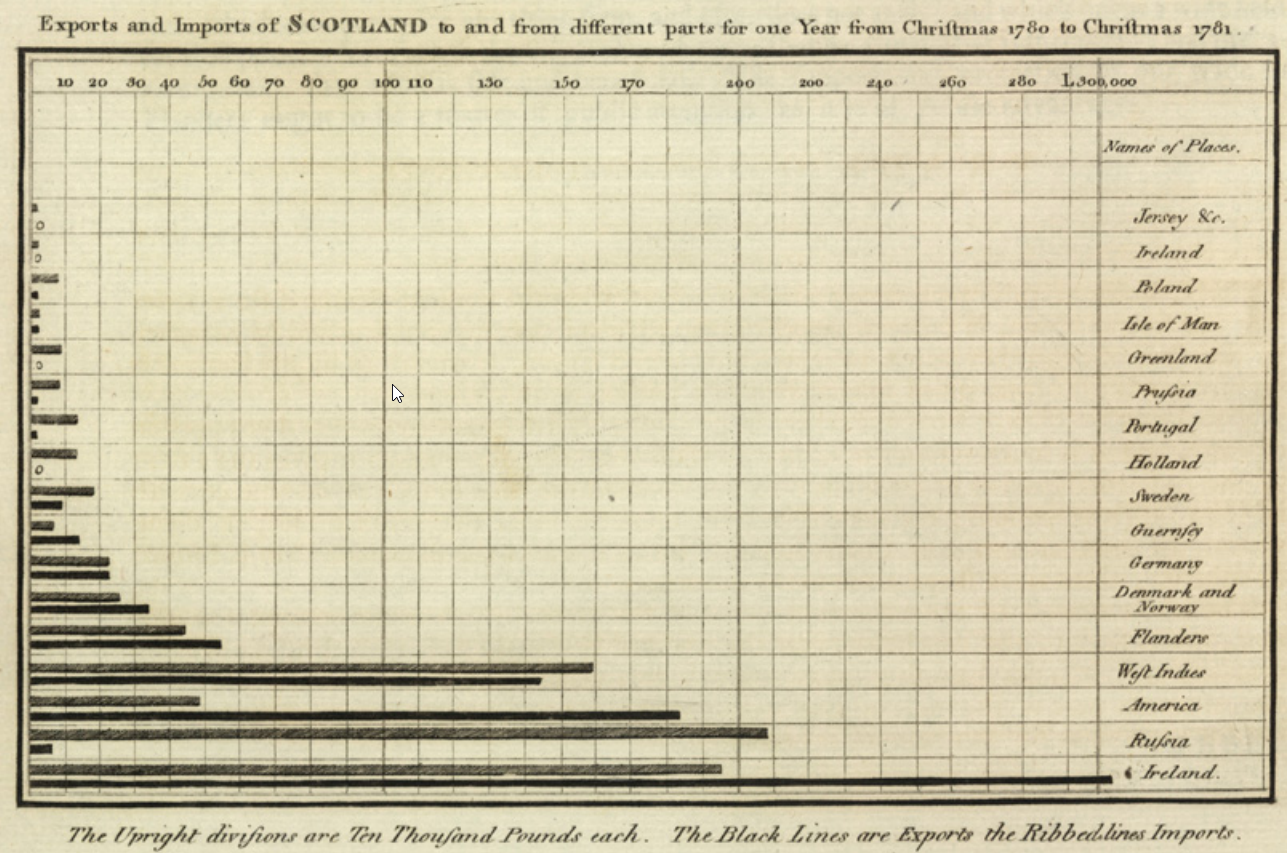
\includegraphics[keepaspectratio,width=\linewidth,height=\fullh / 3]
    {images/playfair-bar-chart.png}
    \caption[Bar Chart by William Playfair from 1786]{
        This chart shows England's exports and imports from and to Scotland in 1781 visualized as a bar chart. It was published in 1786 and is considered to be one of the first occurrences of a bar chart that contains all components found in modern visualizations. \imgcredit{Image extracted from Schoenberg Center for Electronic Text and Image (SCETI). Used under the terms of Creative Commons CC BY 2.5.}
    }
    \label{fig:PlayfairBarChart}
\end{figure}

\begin{figure}[tp]
    \centering
    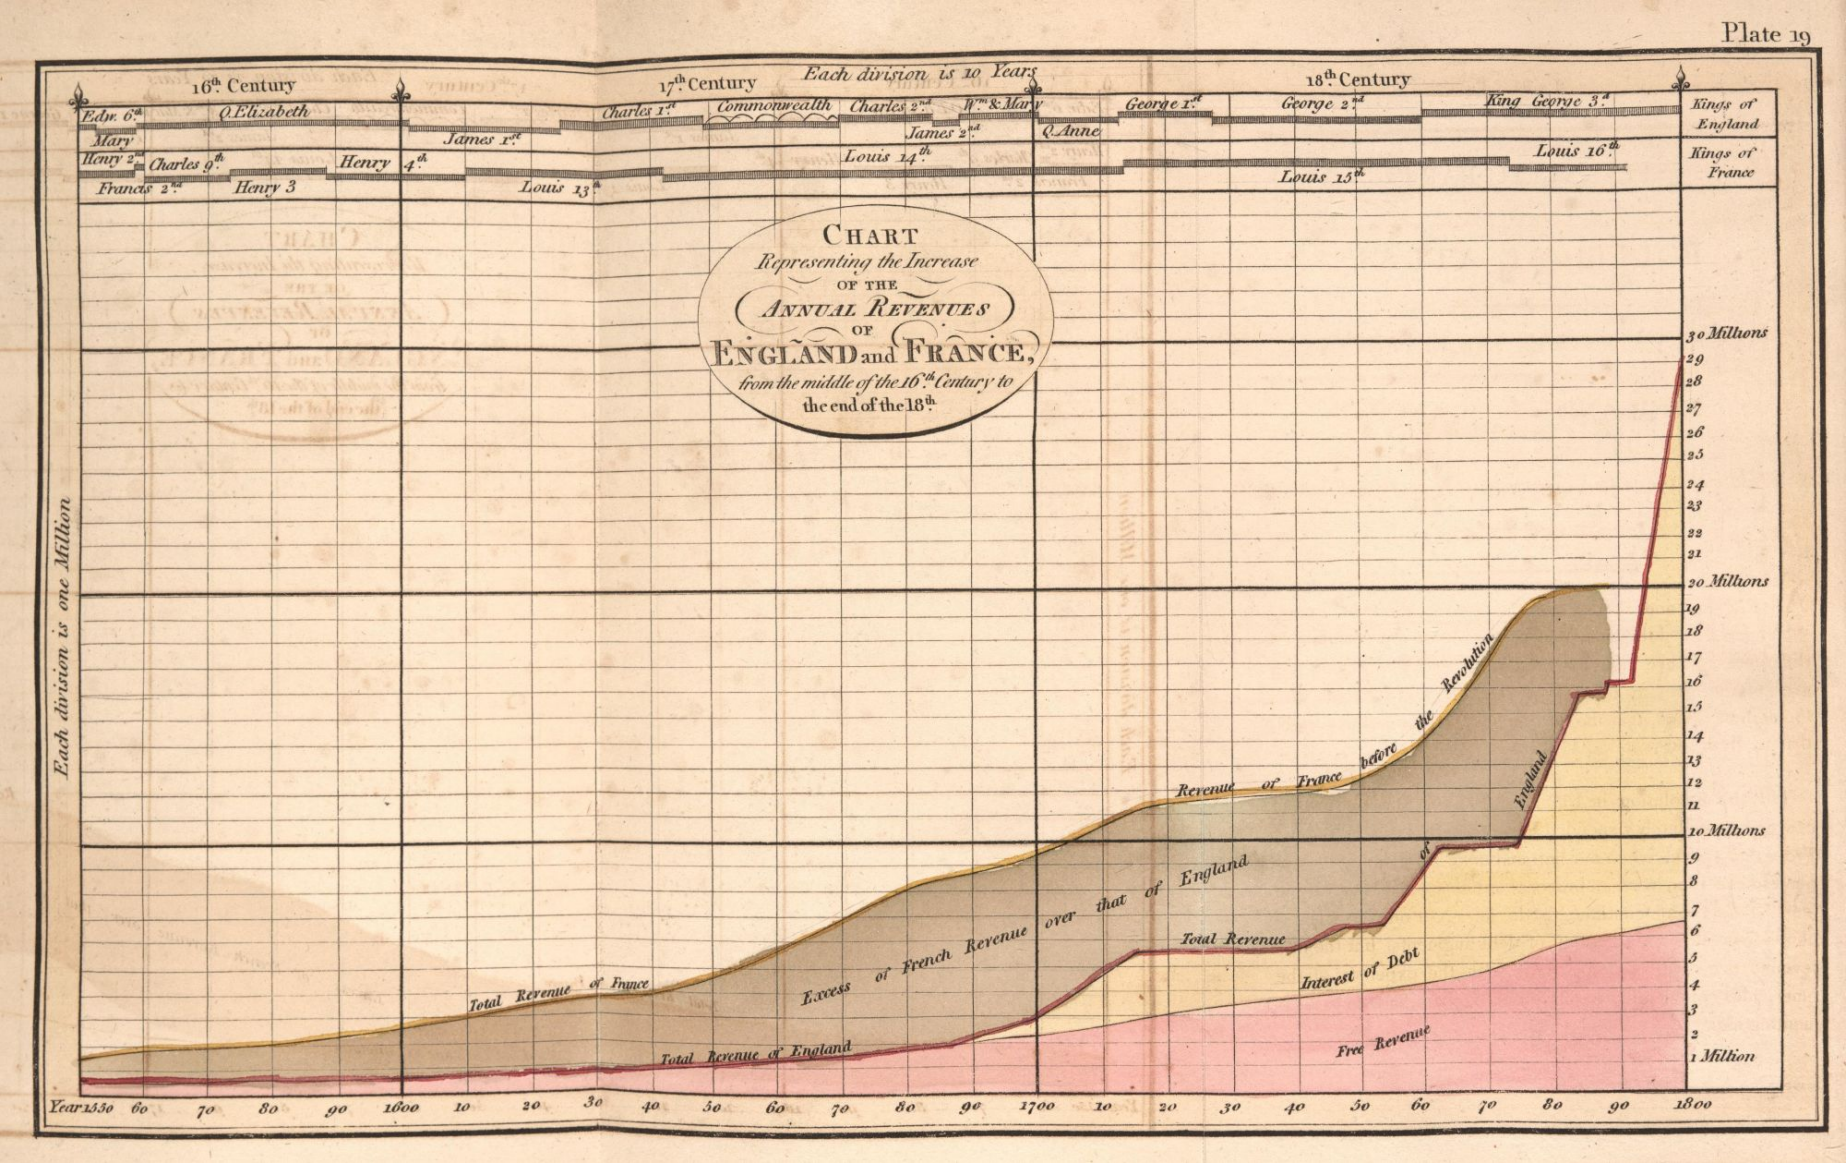
\includegraphics[keepaspectratio,width=\linewidth,height=\fullh / 3]
    {images/playfair-area-chart.png}
    \caption[Area Chart by William Playfair from 1786]{
        This chart shows the annual revenues of England and France between 1550 and 1800 visualized as an area chart. It was published in 1786 and is considered to be one of the first occurrences of an area chart that contains all components found in modern visualizations. \imgcredit{Image extracted from Schoenberg Center for Electronic Text and Image (SCETI). Used under the terms of Creative Commons CC BY 2.5.}
    }
    \label{fig:PlayfairAreaChart}
\end{figure}

Albeit not directly an information visualization but rather a geographic one, the dot map created by \cite{ModeOfCommunicationOfCholera} in 1855 to trace cholera outbreaks in London (Figure \ref{fig:CholeraDotMap}) is undoubtedly one of the most famous and influential visualizations in history. It was used to identify a cluster of cholera-related deaths near a contaminated water pump on Broad Street, leading to the recognition of cholera as a waterborne disease.

\begin{figure}[tp]
    \centering
    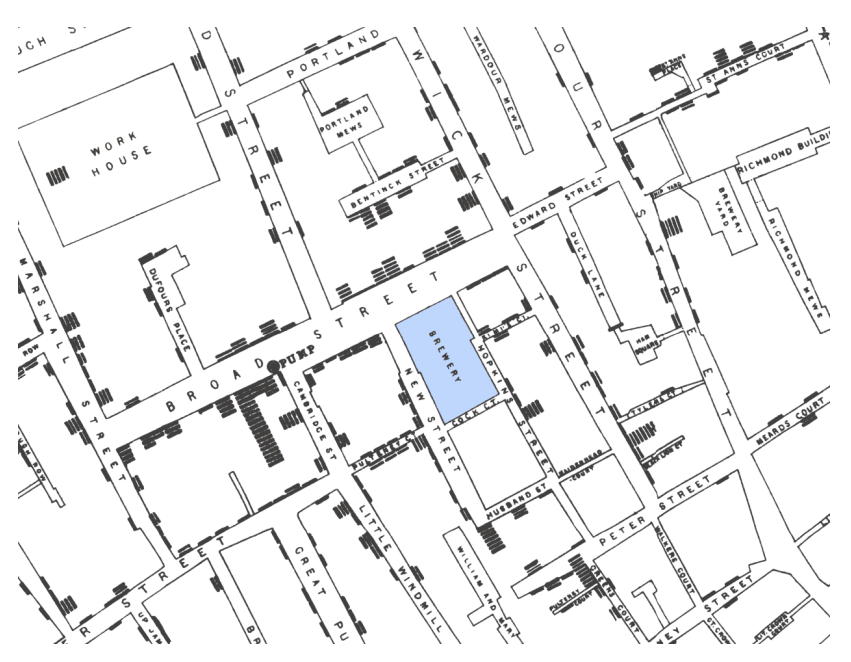
\includegraphics[keepaspectratio,width=\linewidth,height=\fullh / 3]
    {images/cholera-dot-map.png}
    \caption[Dot Map Plotting Cholera Deaths in London From 1855]{
        This iconic chart was created by Dr. John Snow in 1855 to identify a clustering of cholera-related deaths near Broad Street in London. It was used to identify a contaminated water pump and to illustrate the waterborne nature of the disease. The data being map-based, this chart is an example of a data visualization rather than an information visualization. \imgcredit{Image extracted from \cite{IVISCourseNotes}. Original appearance in \cite{ModeOfCommunicationOfCholera}.}
    }
    \label{fig:CholeraDotMap}
\end{figure}

It would go amiss not to mention Florence Nightingale (1820 - 1910) \parencite{FlorenceNightingale} when talking about the history of information visualization. She was a British statistician, social reformer, founder of modern nursing and might be the first person who used visualizations to persuade others of a need for change. During her service as a superintendent of nurses in the Crimean War, she realized that a large share of deaths in hospitals resulted from preventable diseases that originated in poor sanitary conditions. One of her contributions to the field of information visualization was the creation of a new type of diagram, called a rose or polar-area chart. These charts were used to communicate the data she collected on the mortality of soldiers during the war and to grab the attention of politicians and the public. One of those charts can be seen in Figure \ref{fig:NightingalePolarAreaChart}.

\begin{figure}[tp]
    \centering
    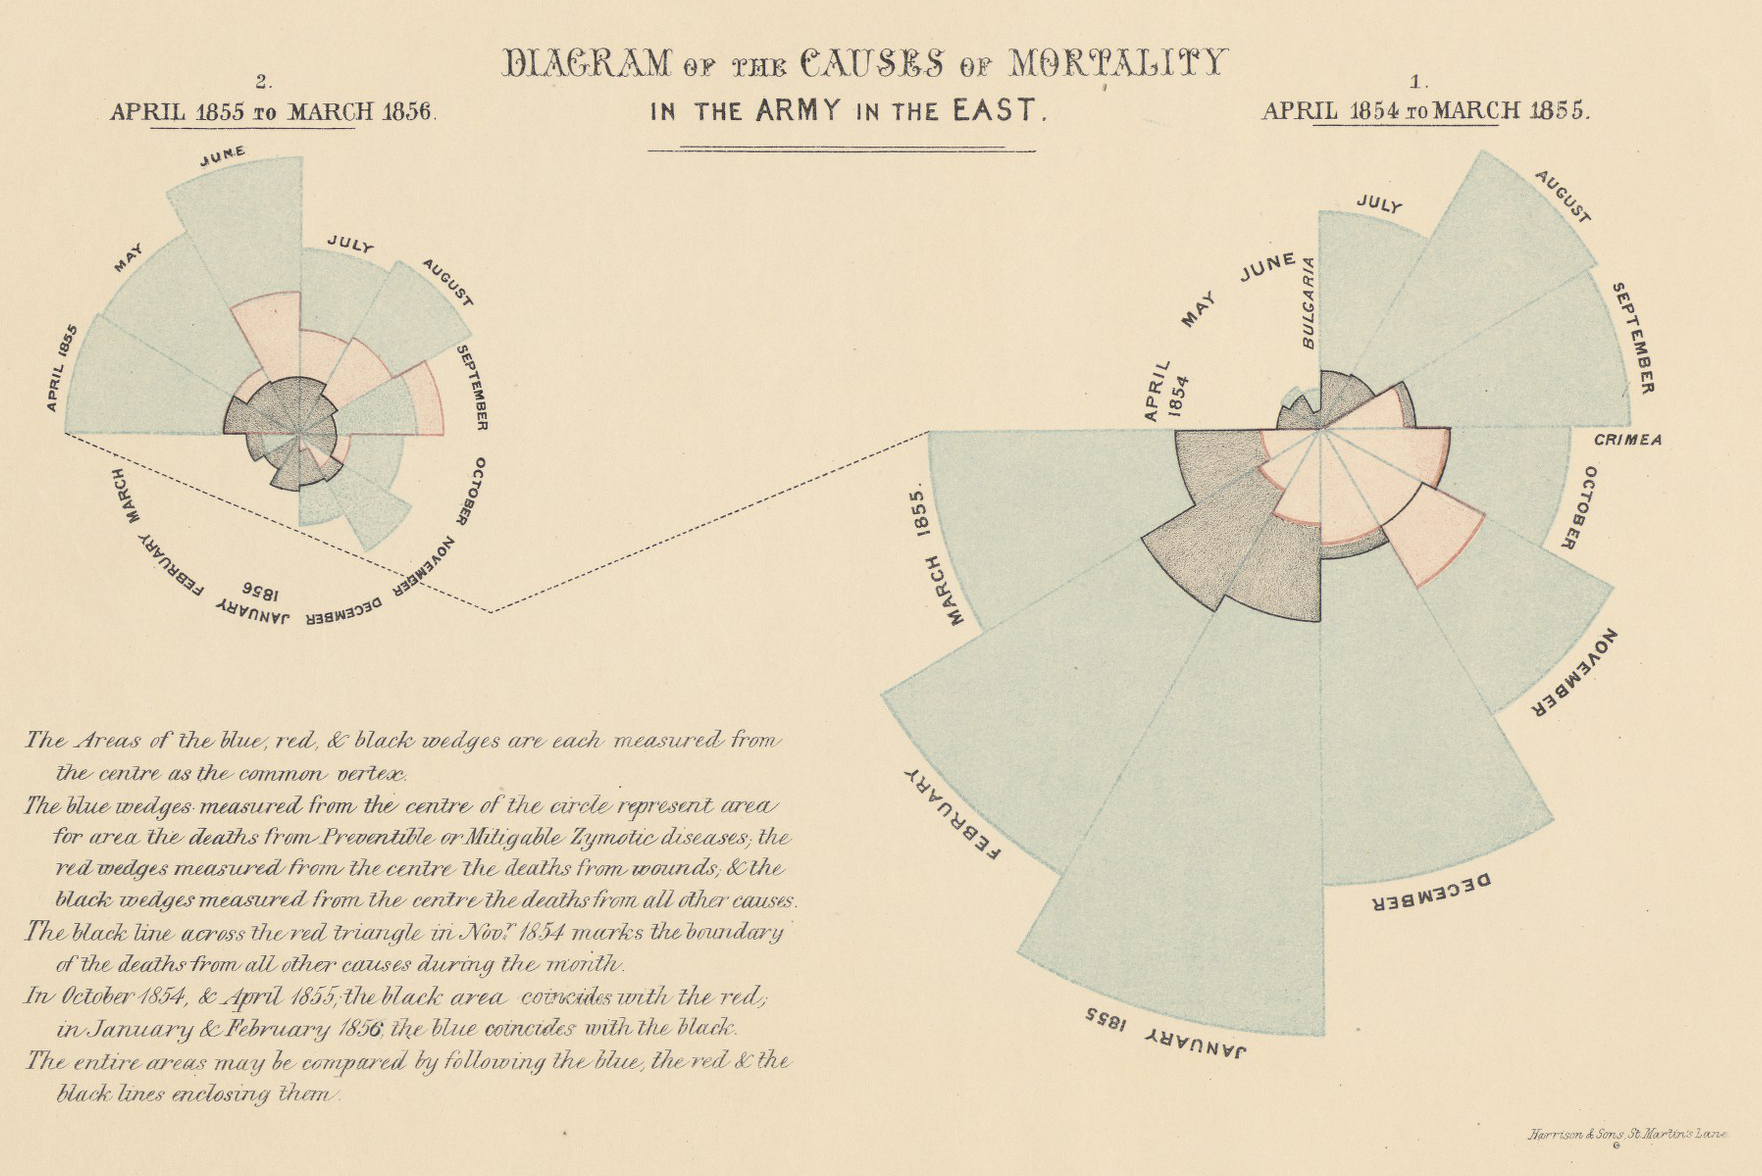
\includegraphics[keepaspectratio,width=\linewidth,height=\fullh / 3]
    {images/nightingale.png}
    \caption[Polar-Area Chart by Florence Nightingale From 1859]{
        This is one of the polar-area charts that Florence Nightingale created in 1859 to convince others of a need for more sanitary conditions in hospitals. It visualizes the causes of mortality for soldiers during the Crimean War and demonstrates that a large percentage of patients died from preventable diseases that are linked to unsanitary environments.
        \imgcredit{Image extracted from Harvard Library. Used under the terms of Creative Commons Attribution 4.0.}
    }
    \label{fig:NightingalePolarAreaChart}
\end{figure}

Modern visualizations benefit from the interactive nature of the devices used to consume them. They are allowed to be a lot more complex than static visualizations because various interaction techniques enable users to navigate large amounts of data and make sense of it. High-D by the company Macrofocus \parencite{HighD} has been chosen as a representative example of such a visual analytics tool and a screenshot of its interface during the analysis of a sample dataset can be seen in Figure \ref{fig:HighD}.

\begin{figure}[tp]
    \centering
    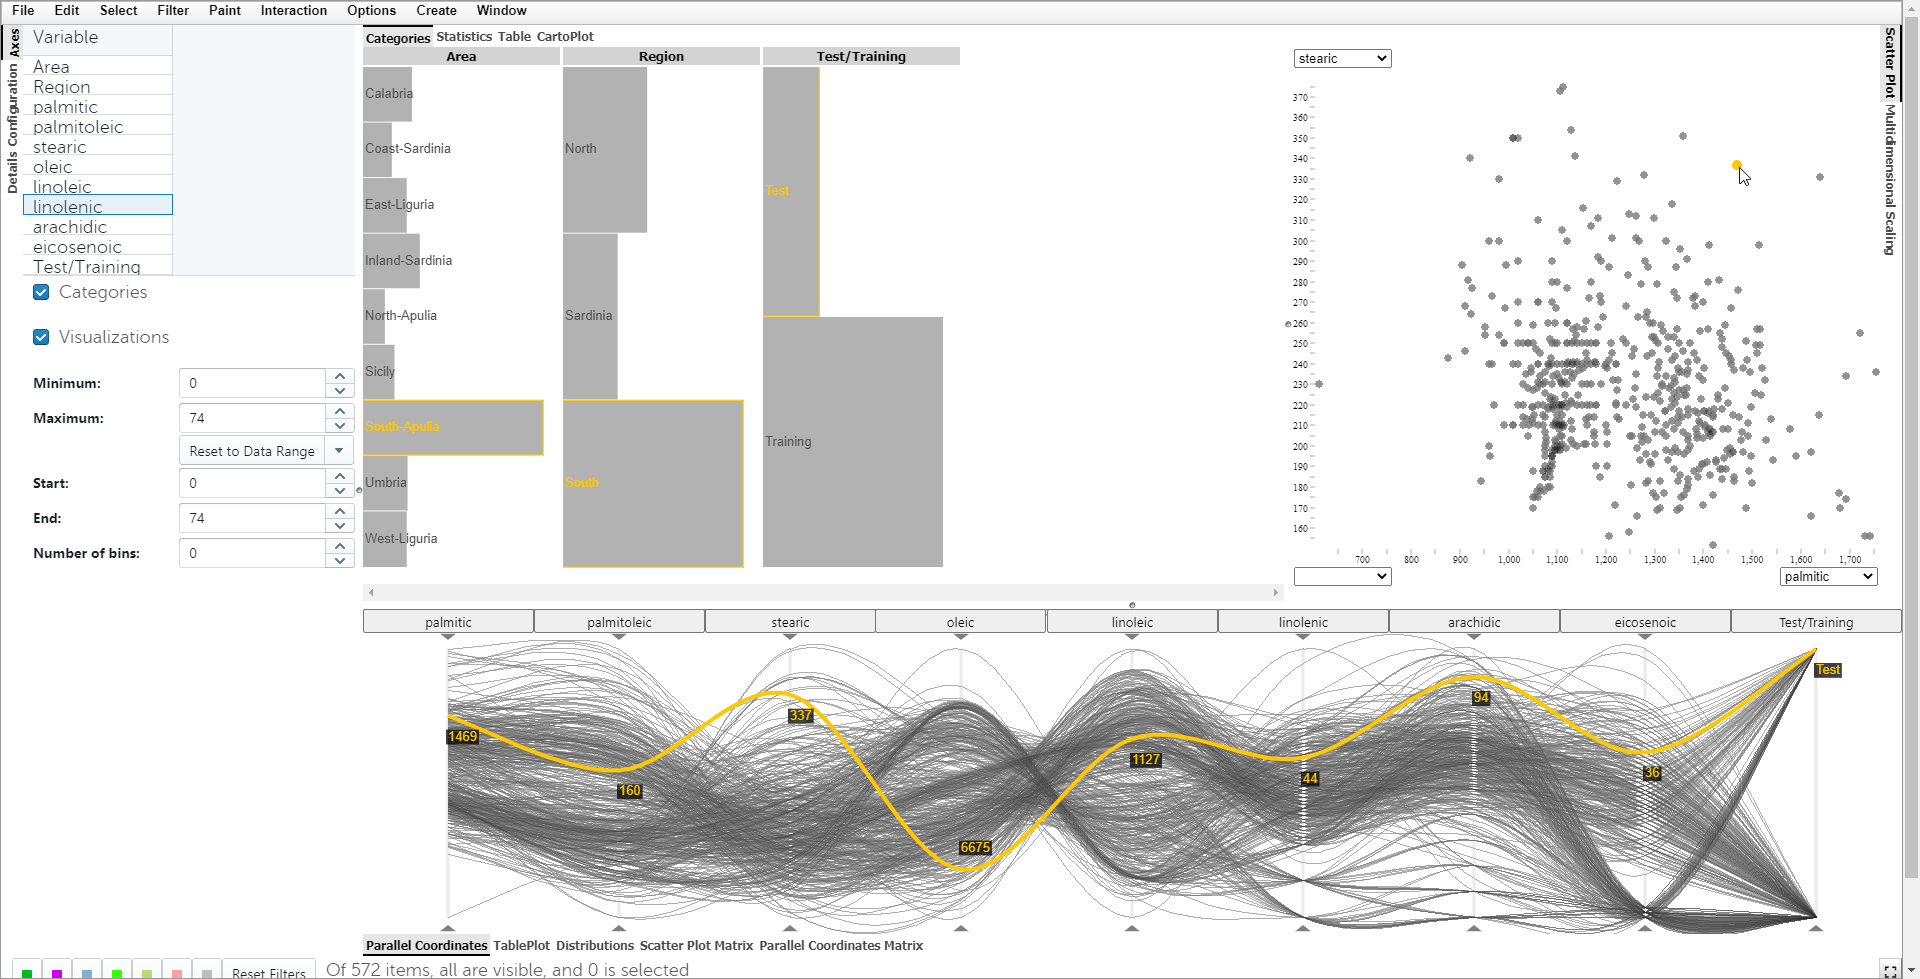
\includegraphics[keepaspectratio,width=\linewidth,height=\fullh / 3]
    {images/high-d.png}
    \caption[Screenshot of High-D]{
        High-D from the company Macrofocus is a visual analytics tool that is specialized in analyzing multidimensional data. 
        \imgcredit{Screenshot of \cite{HighD} taken by the author of this work.} \TODO{How to cite this? Copyright?}
    }
    \label{fig:HighD}
\end{figure}

It is out of the scope of this work to provide a detailed account over the long and eventful history of information visualization and this section only provides a brief and very selective view on the topic. Much more comprehensive works exist that go significantly deeper into details of the various actors and the intricate influences they had on each other. Recommendable sources for further reading on the history of visualization include \cite{BriefHistoryOfDataVis}, \cite{HistoryOfDataVisAndGraphicCommunication} and \cite{HistoryOfInformationGraphics}.

\section{Information Visualization Libraries for the Web}

There are many web-based libraries that simplify the rendering of interactive visualizations. The approaches used to create and update visualization can be vastly different between libraries. D3 is a low-level library that enables data-driven transformations of documents, Vega and Vega-Lite provide a declarative grammar that enables the expression of visual and interactive characteristics of visualizations, and template-based visualization libraries provide a template-based interface that can easily be configured. These libraries and some of their characteristics will be summarized in the following sections.

\subsection{Data-Driven Documents (D3)}

D3 \parencite{D3} is a free and open-source document manipulation library built in JavaScript. It is maintained by an active GitHub community and its core maintainer Mike Bostock who is also the creator of Observable \parencite{Observable} and the deprecated Protovis visualization library \parencite{Protovis}.

D3 enables data-driven document transformations that allow developers to describe their documents as functions of data. As an example, developers can define transformations that receive a dataset and transform it into a basic HTML table or into a more sophisticated visualization as an SVG chart. This focus on explicitly defining transformations is better suited for dynamic visualizations because developers have complete control over the creation, modification and removal of elements. It also sets D3 apart from other visualization libraries where developers usually define the desired state of a representation using a declarative domain specific language.

In contrast to other visualization libraries, D3 contains no proprietary visual primitives and relies on well established web standards like HTML, SVG and CSS to provide visual representations. This yields a lot of flexibility because developers work directly with web standards that are implemented by their browsers and do not need to wait for D3 to implement support for new features as standards evolve. If developers chose to switch to a different library, the knowledge of web standards they gained during their work with D3 might be applicable in their future work. The reliance on web standards also makes it possible to use debugging tools that are already natively implemented in browsers.

Other important aspects of D3's design include immediate evaluation, the principle of parsimony, and support for method chaining. Immediately evaluating functions means that operations, such as modifying attributes, are applied instantaneously at the time of calling the respective functions. This achieves a reduction in internal complexity by handing it over to invoking code and avoids common errors related to missing state changes when state is being modified multiple times between rendering. The principle of parsimony, also referred to as Occam's razor, is a problem-solving principle that stems from the field of philosophy \parencite{PrincipleOfParsimony}. It is frequently paraphrased as "entities should not be multiplied beyond necessity" and when applied to API design it means that superfluous functions in an API should be avoided. As an example, the background color of a circle element can already be set with the generic \lstinline{Selection.attr} method to set the \attrname{background-color} attribute of all elements in a Selection. Adding an additional \lstinline{backgroundColor} method would violate the principle of parsimony. Method chaining is a popular syntax that allows functions to be chained after one another to avoid having to store intermediate results into variables that would otherwise not be needed. It is implemented in D3 by returning the \lstinline{Selection} on which a modifying method is called as a result of that method. Methods that insert new elements into the DOM, such as \lstinline{Selection.append} and \lstinline{Selection.insert}, return a Selection of the newly added elements instead to enable the creation of nested structures. This method chaining syntax is further improved by the \lstinline{Selection.call} method that invokes a callback receiving the current Selection as a parameter and returns the original Selection to further chain methods on it after the callback has been executed. The \lstinline{Selection.call} method enables the creation of complex method chaining structures and is widely used by developers. A simple example of method chaining in D3 and the application of the \lstinline{Selection.call} method can be seen in Figure \ref{list:D3MethodChaining}.

\begin{samepage}
\lstinputlisting[%
  float=tp,
  aboveskip=\floatsep,
  belowskip=\floatsep,
  xleftmargin=0cm,              % no extra margins for floats
  xrightmargin=0cm,             % no extra margins for floats
  %
  language=JavaScript,
  basicstyle=\footnotesize\ttfamily,
  frame=shadowbox,
  numbers=left,
  label=list:D3MethodChaining,
  caption={
    [D3 Method Chaining] A simple example of method chaining in D3 that creates an \elname{h1} and \elname{p} element inside a \elname{body}.
  },
]{listings/d3-method-chaining.js}
\end{samepage}

Selections have already been mentioned in the previous paragraphs. They are the atomic building blocks of D3 that are used to access almost any functionality. Selections are created using the \lstinline{d3.select} or \lstinline{d3.selectAll} methods. These methods are built on the DOM Selectors API, namely the \lstinline{querySelector} and \lstinline{querySelectorAll} methods, which allow the selection of elements via CSS selectors (see Section \ref{sec:CSS}), and which consequentially allow the \lstinline{d3.select} and \lstinline{d3.selectAll} methods to either create a Selection containing a single element matching the provided selector or to create one that contains multiple elements matching it. A Selection acts as a wrapper container around these selected elements, and it provides methods to perform frequently performed DOM operations on them. Among others, the element operations provided by a Selection include the setting and getting of: Attributes using the \lstinline{Selection.attr} method, styles using the \lstinline{Selection.style} method, properties using the \lstinline{Selection.property} method, text or HTML content using the \lstinline{Selection.text} or \lstinline{Selection.html} methods, and event listeners using the \lstinline{Selection.on} method. Selections also provide wrapper methods to add additional elements to the document using the \lstinline{Selection.append} or \lstinline{Selection.insert} methods as well as to remove them using the \lstinline{Selection.remove} method. Accessing the DOM using these methods is less tedious because the API that is natively provided by the DOM is very verbose and also because the method chaining API provided by D3 does not require intermediate variables where none are needed.

An additional feature that D3 adds is the ability to bind data to elements using the \lstinline{Selection.data} and \lstinline{Selection.datum} methods. The \lstinline{Selection.datum} method binds a single provided data record to all elements in the Selection, whereas the \lstinline{Selection.data} method receives an array of data records and binds each individual data record to exactly one element. The \lstinline{Selection.data} method performs a join operation between data and elements to ensure that exactly one element per data record exists. This data join results in three separate Selections: the enter Selection, containing the elements that were newly created, the update Selection, containing the elements that merely receive new data, and the exit Selection, containing the elements that are being removed. Each of these Selections can be individually transformed using the \lstinline{Selection.join} method, which can receive three callbacks each being respectively invoked with the enter, update and exit Selections of the data join. This ability of individually controlling updates of entering, updating and exiting elements is being referred to as the general update pattern in D3 and a simple demonstration of how it is used can be seen in Figure \ref{list:D3GeneralUpdatePattern}. All the previously mentioned DOM wrapper methods can receive either constant values or dynamic ones that are defined as functions. These functions receive the bound element data, the element's index in the group of nodes represented by the Selection, and the group of nodes themselves as input and calculate a dynamic value based on these parameters, which is then forwarded to the corresponding DOM methods. 

\begin{samepage}
\lstinputlisting[%
  float=tp,
  aboveskip=\floatsep,
  belowskip=\floatsep,
  xleftmargin=0cm,              % no extra margins for floats
  xrightmargin=0cm,             % no extra margins for floats
  %
  basicstyle=\footnotesize\ttfamily,
  frame=shadowbox,
  numbers=left,
  label=list:D3GeneralUpdatePattern,
  caption={
    [D3 General Update Pattern] A demonstration of D3's general update pattern and how it can be used to specify different transformations for entering, updating and exiting elements.
  },
]{listings/d3-join.js}
\end{samepage}

D3 also offers a convenient and optional API to perform JavaScript-based animations via Transitions, which wrap a Selection and allow the animation of various element characteristics. 
Transitions are created using the \lstinline{Selection.transition} method that creates a Transition wrapping the Selection on which it has been called. 
The duration of a Transition is defined using the \lstinline{Transition.duration} method, it's easing can be configured using the \lstinline{Transition.ease} method, and there is also the possibility of interrupting and chaining transitions, but explaining these things would be to go into too many details. Transitions provide an (almost) identical API to Selections. The major change is that the wrapping methods interpolate towards their target values using the set easing function over the set duration instead of setting the target value directly. Using D3 Transitions is completely optional and users can also choose to use other animation technologies, like CSS transitions and animations, instead.

At the core, D3 is simply a low-level library to perform data-driven document transformations. 
Even though this generic core technology is applicable to a wide range of use cases, D3 has been created with a focus on creating visualizations.
Many additional modules exist that simplify performing the higher-level tasks necessary for the rendering of visualizations and despite these functionalities being split on multiple modules, they all follow the same patterns inherent to D3 like method chaining. 
Most modules are implemented as configurable functions that are configured using chainable functions and which can be invoked after configuration to perform a specific action.
Listing all available modules here would be out of the scope of this work, but some noteworthy and characteristic ones include: \modname{d3-shape} to create visual primitives like lines and areas, \modname{d3-scale} to encode abstract data dimensions, \modname{d3-axis} to render scales as human-readable axes, and many more such as \modname{d3-array}, \modname{d3-layout} and \modname{d3-zoom}.

\subsection{Vega and Vega-Lite}

Vega \parencite{Vega} is a library that consists of a grammar to describe interactive graphics and a parser that translates specifications written in this grammar into static images or web-based views built on SVG documents or the Canvas Web API. 
An interactive visualization in Vega is fully described by a specification written in Vega's grammar, which is a domain specific language designed for the declarative denotation of interactive graphics. 
The syntax of this grammar is based on JavaScript Object Notation (JSON), an easy-to-read format for data serialization that is among the most frequently used textual serialization formats. 
It builds on previous research in the field of declarative visualization design \parencite{GrammarOfGraphics} and, in addition to describing visual appearances, it also contains powerful capabilities to declaratively describe interactions \parencite{ReactiveVega}. 

The visual aspects of a visualization are described in a grammar similar to the one defined by \cite{GrammarOfGraphics}. 
At its top level, a Vega specification contains properties to configure sizing and padding of the container of a visualization. 
Every specification will also contain a data section that either defines data or specifies where to load it from. 
The Vega grammar also supports various forms of data transformation that can successively be applied to a dataset to perform various transformations like filtering, deriving additional fields or deriving additional datasets.
In a majority of cases, these datasets will contain abstract information that requires being mapped to visual properties.
This mapping is configured and performed using scales. 
Vega already contains a variety of scales to help with mapping abstract values to visual properties, and they can broadly be categorized into quantitative scales that map quantitative inputs to quantitative outputs, discrete scales that map discrete inputs to discrete outputs, and discretizing scales that map quantitative inputs to discrete outputs.
For spatially encoded dimensions, these scales can be visualized as axes, whereas non-spatial encodings such as encodings as colors, sizes or shapes can be visualized as legends.
At the core of every visualization lies the encoding of data as visual primitives, which is achieved in Vega via marks.
Marks use scales to encode data fields as properties of their shapes.
Based on D3's general update pattern, the encoding of marks can be separately controlled for newly created (entering) marks, existing and not exiting (updating) marks, and to-be-removed (exiting) marks.  
In addition to these basic visualization components, the Vega grammar contains further capabilities to describe interactions (via signals, triggers and event streams), cartographic projections, sequential or layered views (via mark groups), layouts and color schemes. 
To demonstrate how the various aspects of a Vega specification are defined, an example that represents a basic bar chart can be seen in Listing \ref{list:VegaStaticBarChart}.

\begin{samepage}
\lstinputlisting[%
  float=tp,
  aboveskip=\floatsep,
  belowskip=\floatsep,
  xleftmargin=0cm,              % no extra margins for floats
  xrightmargin=0cm,             % no extra margins for floats
  %
  basicstyle=\footnotesize\ttfamily,
  frame=shadowbox,
  numbers=left,
  label=list:VegaStaticBarChart,
  caption={
    [Static Bar Chart in Vega] The Vega specification of a static bar chart. 
    Demonstrates the principle of data, scales, axes and marks.
  },
]{listings/vega-static-bar-chart.json}
\end{samepage}

In template-based visualization libraries, interactions are typically defined by configuring premade interaction templates, which is easy but limiting, or by manually modifying the visualization in various callbacks, which is flexible but tedious and not serializable.
The ability to describe custom interactions using a serializable, data-driven grammar is what sets Vega apart from other declarative visualization libraries because it offers a comparable flexibility to callback-driven interactions while still remaining fully serializable and declarative. 
The grammar to define interactions is based on the syntax of event-driven functional reactive programming \parencite{EventDrivenFRP}, a high-level grammar that resembles mathematical equations to describe reactive systems.
In Vega, the primitives to express interactions are called signals. 
Signals can be seen as dynamic variables that can change their values based on input events or other signals. 
These signals and the way their values change are declaratively defined, and they can be used as dynamic variables throughout most places in a Vega specification to change various characteristics of a visualization dynamically. 
An example of how the previously demonstrated bar chart specification can be extended with signals to show a tooltip when hovering bars can be seen in Listing \ref{list:VegaBarChart}. 

\begin{samepage}
\lstinputlisting[%
  float=tp,
  aboveskip=\floatsep,
  belowskip=\floatsep,
  xleftmargin=0cm,              % no extra margins for floats
  xrightmargin=0cm,             % no extra margins for floats
  %
  basicstyle=\footnotesize\ttfamily,
  frame=shadowbox,
  numbers=left,
  label=list:VegaBarChart,
  caption={
    [Bar Chart with Tooltip in Vega] The necessary changes to the bar chart specification in Listing \ref{list:VegaStaticBarChart} to add show a tooltip when hovering over bars. It demonstrates the basic functionality of signals in Vega. When the mouse hovers over a rect mark, the tooltip signal will receive the value of the rect's bound data record and when the mouse leaves the rect mark, the variable will be reset to an empty object. The tooltip signal is then used in the newly added text mark to define the position, text and visibility of it whenever an update occurs.
  },
]{listings/vega-bar-chart.json}
\end{samepage}

Visualizations created with Vega closely follow their specifications and minimal assumptions are being made in the compilation process. This results in very verbose specifications because all configurations for all parts of the visualization need to be explicitly defined in them. It also means that specification authors have full control over the resulting graphics, which makes Vega a good base on which to build further libraries and tools. Many tools \parencite{Voyager,Lyra,CompassQL} have been built on top of Vega but the one worth mentioning most is Vega-Lite \parencite{VegaLite}. Vega-Lite is described as a "high-level grammar of interactive graphics", which summarizes its difference to Vega fairly well. Compared to Vega, Vega-Lite is a higher-level grammar that allows authors to write specifications for common visualizations in a much more concise form. Specifications written in Vega-Lite are compiled into Vega specifications and the compiler automatically derives default configurations for axes, legends and scales from a set of carefully designed rules. This makes Vega-Lite more convenient to use for quick authoring of visualizations because many details that need to be explicitly stated in a Vega specification can be omitted. Vega-Lite also offers the possibility to override derived defaults and, because Vega-Lite specifications are simply being compiled into Vega ones, it is a sensible choice to use Vega-Lite as a primary tool to describe visualizations and switch to Vega for more exotic cases that are not easily achievable in Vega-Lite. To properly compare the difference between Vega and Vega-Lite specifications, a Vega-Lite version of the Vega bar chart specification seen in Listing \ref{list:VegaStaticBarChart} can be seen in Listing \ref{list:VegaLiteBarChart}.

\begin{samepage}
\lstinputlisting[%
  float=tp,
  aboveskip=\floatsep,
  belowskip=\floatsep,
  xleftmargin=0cm,              % no extra margins for floats
  xrightmargin=0cm,             % no extra margins for floats
  %
  basicstyle=\footnotesize\ttfamily,
  frame=shadowbox,
  numbers=left,
  label=list:VegaLiteBarChart,
  caption={
    [Bar Chart with Tooltip in Vega-Lite] This is a Vega-Lite specification of the Vega bar chart specification seen in Listing \ref{list:VegaStaticBarChart} combined with Listing \ref{list:VegaBarChart}.
  },
]{listings/vega-lite-bar-chart.json}
\end{samepage}

\subsection{Template-Based Visualization Libraries}

Template-based visualization libraries work by providing templates for possible types of visualizations and allowing users to customize them. 
These types of visualization libraries are easier to use than D3 or Vega because they offer a concise form of configuration that does not require users to have detailed knowledge over the underlying rendering technology or complex, non-standardized domain specific languages. 
Even though these types of libraries are usually very flexible and suited to create a huge range of visualizations, at one point users may run into limitations that can not be worked around without writing custom source code that requires a deep understanding of the underlying library. 

For this thesis, a total of 20 template-based JavaScript visualization libraries have been collected and compared by different factors such as their rendering technology, usage popularity, open-source popularity, license, and recent development activity. 
In terms of rendering technology, most libraries render visualizations as either SVG documents or canvas elements, though some implement a hybrid renderer that can be configured to render as either one of them. 
Usage popularity has been measured by the cumulative package downloads from the npm package manager over the last twelve months. 
This has been deemed one of the most relevant metrics for the comparison because it reflects actual user behavior and gives an indication of how widespread a library is used in practice. 
The 20 libraries that were found in the initial collection phase were filtered by their usage popularity and recent development activity to remove those that were not sufficiently used or maintained anymore. 
This filtering step yielded the following ten libraries: (1) ChartJS \parencite{ChartJS}, (2) Highcharts \parencite{Highcharts}, (3) ECharts \parencite{ECharts}, (4) ApexCharts \parencite{ApexCharts}, (5) PlotlyJS \parencite{PlotlyJS}, (6) C3JS \parencite{C3JS}, (7) Chartist \parencite{Chartist}, (8) amCharts \parencite{amCharts}, (9) billboardJS \parencite{billboardJS}, and (10) D3FC \parencite{D3FC}. 
These libraries have been selected for deeper evaluation because they are heavily used and, for the most part, still actively maintained. 
The focus of this more detailed analysis is on summarizing these libraries based on high-level features and responsive capabilities.

Eight of those ten libraries are completely free to use without restrictions, amCharts has a free license for users that are comfortable with an attribution logo on their visualizations, and Highcharts offers a free license option for non-profit, educational and personal applications.
Nine libraries implement a renderer that is based on SVG, two of which (ECharts, D3FC) offer alternative rendering to canvas elements for high-performance scenarios, and only ChartJS purely targets canvas-based rendering. 
Eight libraries are very actively maintained with most of them showing development activity within the last month. 
Only C3JS and Chartist do not seem to be actively maintained anymore, but they nonetheless have been included in the deeper evaluation because of their historic and thematic relevance and because they are still widely used. 

Similar to Vega, template-based visualization libraries have a strong inclination towards designing their APIs according to principles of declarative programming. 
APIs following these principles allow users to describe a desired state they want the underlying system to be in. 
This is in strong contrast to the typical imperative way of designing APIs in which users are instead given a set of tools to query and modify a system's state. 
The difference can be summarized in simple terms as: Using declarative APIs, users specify what state shall be achieved, whereas when using imperative APIs, users specify how a certain state is achieved. 
Declarative APIs are typically built on top of lower-level imperative APIs and can therefore be seen as a higher level of abstraction over them. 
They are popular among developers because they are expressive, easy to use and effectively encapsulate complexity that would otherwise have to be handled by users. 
A disadvantage of declarative APIs that is often overlooked is that they frequently only provide high-level access to a system and that more specific use cases might not be achievable if they can not be expressed in the domain specific language defined by the API. 
In many cases it makes sense to provide additional (optional) imperative APIs so that users requiring a lower level of access to the system can implement functionality not achievable via the declarative parts of the interface.

All evaluated libraries, except D3FC, expose declarative interfaces in the form of nested configuration objects that are used to specify the characteristics of individual visualizations. 
Apart from Chartist, all those libraries feature generic high-level functions that create charts from declarative configuration objects that allow the specification of different forms of visualization for different data dimensions. 
This type of interface is demonstrated by the Highcharts code seen in Listing \ref{list:Highcharts}. 
These generic chart creation functions seem to be correlated with the ability of dynamically changing the type of visualization. 
In Chartist, for instance, which provides separate chart creation functions for each type of chart, it is not possible to alter the type of chart after it has been created. 
Another limitation that may originate in this interface partitioning via chart types is that mixed charts that combine multiple forms of visualization in one composite visualization can not be expressed. 
The only library in the deeper evaluation that does not provide a high-level declarative configuration API is D3FC. 
The design philosophy of D3FC is based on the idea of "unboxing" D3 because even though many visualization libraries are implemented on top of D3, it is usually hidden behind public APIs that are easier to work with but don't provide the full flexibility that D3 does. 
D3FC exposes a component-based interface that closely follows design patterns frequently encountered when working with D3. 
These components form higher-level building blocks on which advanced visualizations can be built. 
They are also highly configurable and in those cases where the options for configuration are not sufficient, a decorator pattern is used to allow users to hook into the underlying D3 functionality and inject custom code into the various stages of the general update pattern at the core of D3.
Code that demonstrates the usage of D3FC can be seen in Listing \ref{list:D3FC}. 
The only evaluated library that exposes a hybrid API with the possibility of configuring visualizations using both declarative configuration objects and manually composing higher-level visualizations from lower-level components, such as axes and series, is amCharts.
Its component-based interface is still rather declarative, with most options being configurable by modifying certain properties on the components.
However, modifying only the properties that require changing instead of processing a full configuration object and figuring out the necessary changes from it is less costly in terms of performance. 
In addition to these performance benefits, the components provide additional functions to perform operations that would not be available using a purely declarative API.

\begin{samepage}
\lstinputlisting[%
  float=tp,
  aboveskip=\floatsep,
  belowskip=\floatsep,
  xleftmargin=0cm,              % no extra margins for floats
  xrightmargin=0cm,             % no extra margins for floats
  %
  basicstyle=\footnotesize\ttfamily,
  frame=shadowbox,
  numbers=left,
  label=list:Highcharts,
  caption={
    [Bar Chart in Highcharts] This example demonstrates how a basic column (vertical bar) chart is defined using the generic chart creation API provided by Highcharts.
  },
]{listings/highcharts.js}
\end{samepage}

\begin{samepage}
\lstinputlisting[%
  float=tp,
  aboveskip=\floatsep,
  belowskip=\floatsep,
  xleftmargin=0cm,              % no extra margins for floats
  xrightmargin=0cm,             % no extra margins for floats
  %
  basicstyle=\footnotesize\ttfamily,
  frame=shadowbox,
  numbers=left,
  label=list:D3FC,
  caption={
    [Bar Chart in D3FC] This example demonstrates how a basic bar chart is defined using the component-based API provided by D3FC.
  },
]{listings/d3fc.js}
\end{samepage}

When comparing the evaluated libraries by their responsive configurability, most libraries offer similar capabilities albeit in slightly different ways.
Six libraries (Highcharts, C3JS, Chartist, amCharts, billboardJS, D3FC) support the styling of elements in their created visualizations with CSS, which requires rendering as SVG documents because only document-based visualizations can be affected by CSS.
The styling of visualizations with CSS is powerful because it leads to a separation of concerns and designers can make use of CSS-inherent mechanisms to configure responsive styles.
Unfortunately, CSS-based styling is only of limited applicability because not all CSS properties affect SVG elements, which has already been described in Section \ref{sec:SVG}.
To responsively configure other visualization characteristics, such as their type, data, and layout, designers have to resort to configuration mechanisms offered by the libraries. 
Four libraries (Highcharts, ApexCharts, Chartist, amCharts) provide the possibility to specify rule-based responsive configurations as part of their declarative interfaces, demonstrated in the Highcharts example in Listing \ref{list:HighchartsResponsive}.
These declarative rules consist of a condition part that specifies when to apply the rule, and a configuration part that specifies the configuration options that should be set when applying the rule.
Even though this is a convenient form of responsive configuration, if the desired conditions can not be expressed via the provided declarative properties, designers have to fall back to more generic mechanisms that are also applicable to other libraries. 
The mechanisms for responsive configuration in the other libraries are more generic because they don't offer these configurations as part of their declarative interfaces. 
This means that developers need to trigger responsive configurations themselves by manually reconfiguring visualizations via their APIs in custom resize or media query event listeners.
Nearly all libraries provide means to dynamically resize visualizations and update their data, type and options.
The exceptions from this are C3JS, which only supports dynamic changes of some options, and Chartist, which does not support changing of a visualization's type.

\begin{samepage}
\lstinputlisting[%
  float=tp,
  aboveskip=\floatsep,
  belowskip=\floatsep,
  xleftmargin=0cm,              % no extra margins for floats
  xrightmargin=0cm,             % no extra margins for floats
  %
  basicstyle=\footnotesize\ttfamily,
  frame=shadowbox,
  numbers=left,
  label=list:HighchartsResponsive,
  caption={
    [Responsive Rules in Highcharts] This example demonstrates how responsive rules can be declared to configure various aspects of a visualization in relation to the size of the viewport.
  },
]{listings/highcharts-responsive.js}
\end{samepage}          %   Chapter 3

\cleardoublepage
\chapter{Software Architecture}

\label{chap:SoftwareArchitecture}

\TODO{Add software architecture diagram}


\TODO{Describe relationship to D3}

\TODO{Describe storing data on elements}

\TODO{Describe using DOM events for callbacks}

\TODO{Describe components}

\section{Primitives}

\subsection{Text}

\subsection{Rectangle}

\subsection{Circle}

\section{Series}

\TODO{Describe series extension mechanism (enter/update/exit events)}

\subsection{Bar Series}
\subsection{Grouped Bar Series}
\subsection{Stacked Bar Series}
\subsection{Point Series}
\subsection{Line Series}

\section{Charts}

\subsection{Bar Chart}
\subsection{Grouped Bar Chart}
\subsection{Stacked Bar Chart}
\subsection{Point Chart}
\subsection{Line Chart}

\section{Chart Windows}

\subsection{Bar Chart Window}
\subsection{Grouped Bar Chart Window}
\subsection{Stacked Bar Chart Window}
\subsection{Point Chart Window}
\subsection{Line Chart Window}

\section{Components}



\subsection{Lifecycle}

events

updating on data change

updating on bounds change

\section{Layouter}       %   Chapter 4

\cleardoublepage
\chapter{Modules}
\label{chap:Modules}

\section{Core}

\subsection{Utilities}
\subsection{Selection}
\subsection{Layouter}

\section{Legend}

\section{Tooltip}

\section{Bars}

\subsection{Basic Bars}

\subsection{Grouped Bars}

\subsection{Stacked Bars}

\section{Points}          %   Chapter 5

\cleardoublepage
\chapter{Another Chapter; Maybe about Components?}

\label{chap:Components}

  %   Chapter 6

\cleardoublepage
%----------------------------------------------------------------
%
%  File    :  thesis-details.tex
%
%  Author  :  Keith Andrews, IICM, TU Graz, Austria
% 
%  Created :  17 Nov 2004
% 
%  Changed :  17 Nov 2004
% 
%----------------------------------------------------------------

\chapter{Selected Details of the Implementation
(and Test of Extremely
Long Chapter Titles to See How They Work or Not)
}

\label{chap:SelectedDetails}


\chapquote{
The devil is in the detail.
}
{
English proverb.
}


There are often specific details of a project, which involve
particularly much work to get right, but do not form a major part in
the whole scheme of things, so would not generally deserve a chapter
of their own. This chapter is for these details.



\section{First Selected Detail}

The context, the decision process, all the variations that were tried,
and the solution that was finally adopted.



\section{Second Selected Detail}

From some other part of the project. Explaining your reasoning and
choices will help some other poor student, who has to pick up your
work from where you left off.



\section{Using a Table}

An example of using a table can be seen in Table~\ref{tab:BestPubs}.

\begin{table}[tp]
\centering
\begin{tabularx}{\linewidth}{|llrX|}
\hline
Name & Type & Rating & Description \\
\hline
Flann O'Brien &
Irish &
***** &
In the centre of town and easy to find for
marauding tourists. Very smooth Guinness.
\\
\hline
The Office &
English &
***** &
Hidden in the narrow streets of the old town.
Erasmus student night every other Wednesday.
\\
\hline
O'Carolans &
Irish &
*** &
In the centre of town in a small side street next to Flann's.
Small, cosy, but hellishly smoky.
\\
\hline
O'Riginal &
pseudo Irish &
 &
Austrian dive pretending to be an Irish pub.
\\
\hline
\end{tabularx}

\caption[Best Pubs in Graz]
{
The best pubs in Graz.
}
\label{tab:BestPubs}
\end{table}





\section{Using Subfigures}

This example shows how to include vector graphics in the form of PDF
files. It also shows how to use subfigures within a figure.

\begin{figure}[tp]
\centering
\subfloat[][%  the % chars remove implicit spacing
An object has been composed to represent an
abstract version of the clock tower in Graz.
Here, the object is in its initial state.
]
{%
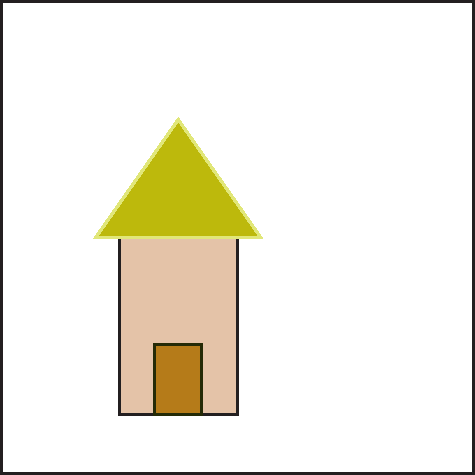
\includegraphics[width=0.45\linewidth]
{diagrams/multi1.pdf}%
\label{fig:Tower1}%
}
\hfill
\subfloat[][%
The object has been scaled and rotated, and now resembles
a leaning tower.
]
{%
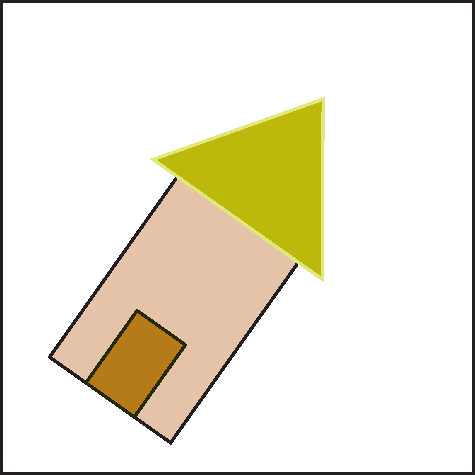
\includegraphics[width=0.45\linewidth]
{diagrams/multi2.pdf}%
\label{fig:Tower2}%
}

\caption[Abstract Clock Towers]
{
The leaning tower of Graz. An abstract model of the clock
tower in Graz leaning over time. \subref{fig:Tower1} shows
the initial state. \subref{fig:Tower2} shows the final state.
\imgcredit{Both images created by the author of this thesis.}
}
\label{fig:WholeFig}
\end{figure}


An example of using the \vname{subfig} package can be seen in
Figure~\ref{fig:WholeFig}. Figure~\ref{fig:Tower1} shows the polygons
before transformation, while Figure~\ref{fig:Tower2} shows them
afterwards.





\section{Including a Screenshot}

This example shows how to include a screenshot (or other raster
graphic) into a \LaTeXe\ figure.

\begin{figure}[tp]
\centering
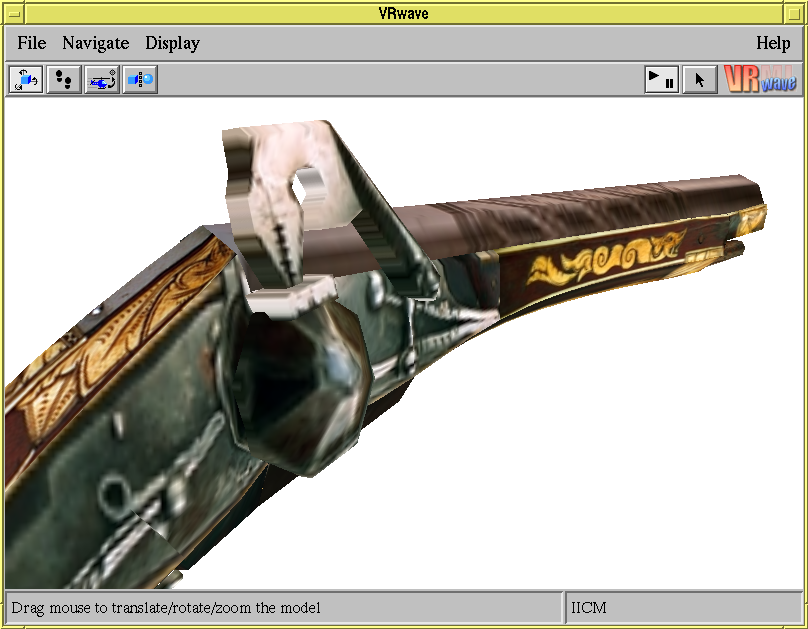
\includegraphics[keepaspectratio,width=\linewidth,height=\halfh]
{images/pist.png}

\caption[VRwave in Flip Mode]
{%
VRwave in Flip mode displaying a textured model of a cavalry pistol
from the world-renowned Zeughaus (armoury) in Graz.
\imgcredit{Image extracted from \textcite[page~81]{Andrews-VRwave}
and used under the terms of the ACM Copyright Policy. \copyrightACM}
}
\label{fig:Pistol}
\end{figure}


An example of how to correctly cite the source when using an image
from someone else. In their 1998 paper, \textcite{Andrews-VRwave}
discuss the VRwave VRML browser. Figure~\ref{fig:Pistol} shows a VRML
model of a cavalry pistol from the Armoury in Graz displayed in the
VRwave VRML browser.





\section{Using Special Characters and Symbols}

You can use many (but not all) of the thousands of characters
available in the UTF-8 \parencites{Wikipedia-UTF8}{Unicode-Charts}
character encoding. For example, the German umlauts (äüö), the German
sharp s (ß), or the yen symbol (¥).

You can also try some of the \approxsym 100 symbols available
in the \vname{textcomp} package, such as the yen symbol (\textyen) and
a circled letter A (\textcircled{A}).



\section{Using Macros to Style Special Names}

Use the \vname{vname}, \vname{cname}, and \vname{fname} macros to
define the style for (say) variable names, class names, and file
names. You can also define your own macros. The is a very long file
name \fname{/usr/data/keith/travel/austria/vienna.txt} to see how they
are broken at a line end. A typical class name is
\cname{HVSInformationPyramidsInputFactory}.





\section{Using Macros as Shorthand}

Sometimes, a macro (new command definition) can be useful to define
the contents of table cells, particularly if these contain images. For
example, Table~\ref{tab:WinIconicLang} uses the macro called
\vname{iibox}, which takes a single parameter, the name of
the particular image.


\begin{table}[tp]

\newcommand{\iibox}[1]{\parbox[c][1cm][c]{1cm}{%
\includegraphics[scale=0.6]{./images/icons/#1.png}
}}

\begin{center}
\begin{tabular}[t]{|p{7cm}c|}
\hline
\multicolumn{2}{|l|}{\sffamily \bfseries Elementary Symbols}            \\
Document                            & \iibox{win-il-gen-doc}            \\
Assistant                           & \iibox{win-il-gen-ass}            \\
Template                            & \iibox{win-il-gen-tmpl}           \\
\hline
\multicolumn{2}{|l|}{\sffamily \bfseries Document Types}                \\
Text document                       & \iibox{win-il-text-doc}           \\
Spreadsheet document                & \iibox{win-il-spreadsheet-doc}    \\
Presentation document               & \iibox{win-il-presentation-doc}   \\
Database document                   & \iibox{win-il-database-doc}       \\
\hline
\multicolumn{2}{|l|}{\sffamily \bfseries Applications}                  \\
Word                                & \iibox{win-il-word-appl}          \\
Excel                               & \iibox{win-il-xls-appl}           \\
Powerpoint                          & \iibox{win-il-ppt-appl}           \\
Access                              & \iibox{win-il-mdb-appl}           \\
\hline
\multicolumn{2}{|l|}{\sffamily \bfseries Generated Icons}               \\
Word text document                  & \iibox{win-il-word-doc}           \\
Excel spreadsheet document          & \iibox{win-il-xls-doc}            \\
Powerpoint presentation document    & \iibox{win-il-ppt-doc}            \\
Access database document            & \iibox{win-il-mdb-doc}            \\[2ex]
%
Word template                       & \iibox{win-il-word-tmpl}          \\
Powerpoint template                 & \iibox{win-il-ppt-tmpl}           \\
Access template                     & \iibox{win-il-mdb-tmpl}           \\[2ex]
%
Word template assistant             & \iibox{win-il-word-ass}           \\
Powerpoint template assistant       & \iibox{win-il-ppt-ass}            \\
Access template assistant           & \iibox{win-il-mdb-ass}            \\[2ex]
%
\hline
\end{tabular}
\end{center}

\caption[Iconic language for Windows NT 4.0 documents]
{
Iconic language for Windows NT 4.0 documents.
\imgcredit{The icons are screenshots, captured and then
enlarged by the author of this thesis.}
}
\label{tab:WinIconicLang}
\end{table}







\begin{samepage}
\begin{lstlisting}[%
  float=tp,
  aboveskip=\floatsep,
  belowskip=\floatsep,
  xleftmargin=0cm,              % no extra margins for floats
  xrightmargin=0cm,             % no extra margins for floats
  basicstyle=\footnotesize\ttfamily,
  frame=shadowbox,
  numbers=left,
  language=HTML,
  label=list:HTML5Boilerplate,
  caption={[HTML5 Boilerplate Code]%
Some HTML5 boilerplate code, illustrating the typical structure
of a HTML5 web page.
},
]
<!DOCTYPE html>
<html xmlns="http://www.w3.org/1999/xhtml" lang="en" xml:lang="en">

<head>
<meta charset="UTF-8"/>
<meta name="viewport" content="width=device-width, initial-scale=1"/>
<link rel="stylesheet" href="./inm.css"/>

<title>Keith Andrews Web Page</title>
</head>

<body>

<header>
<img src="images/kalogo.svg" alt="KA Logo"/>
Keith Andrews Design
</header>

<h1>Keith Andrews</h1>

<p>
Keith lives in <a href="http://graz.at/">Graz</a>.
</p>

<p>
<img src="images/keith-s.jpg"
  alt="Photo of Keith Andrews"/>
</p>

<p>
Three desirable attributes:
</p>
<ol>
<li>cheap</li>
<li>fast</li>
<li>good</li>
</ol>
<p>
Choose any two.
</p>

<p>
<abbr title="Extensible HyperText Markup Language">XHTML</abbr>
is cool.
</p>

<table>
<tbody>
<tr><th>Beer</th><th>Price €</th></tr>
<tr><td>Puntigamer</td><td>2,60</td></tr>
<tr><td>Gösser</td><td>2,60</td></tr>
<tr><td>Guinness</td><td>4,35</td></tr>
</tbody>
</table>

<footer>
Copyright © Keith Andrews 2019.
</footer>

</body>
</html>
\end{lstlisting}
\end{samepage}



\section{Using Floating Listings}

Listing~\ref{list:HTML5Boilerplate} is floating. A floating listing is
a block of code treated like other \LaTeXe floats (such as figures or
tables). Use floating listings for longer blocks of code.
A floating listing is given a number and can be referred to
explicitly, like Listing~\ref{list:HTML5Boilerplate}. It can be given
a caption and short caption, and is listed in the List of Listings.





\section{Using Non-Floating Diplayed Listings}

The listing below shows some CSS:
\begin{samepage}
\begin{lstlisting}[%
  language=CSS,
]
body { color: black; background-color: silver; }
img { border: none; }
h1,h2 { font-family: Verdana, sans-serif; }
\end{lstlisting}
\end{samepage}
It is displayed (i.e. indented as a block) in-place, but is not
floating. It cannot be referred to by number and is not listed in the
List of Listings. As a rule of thumb, if listings have five or more
lines, make them floating.





\section{Using Inline Listings}

Inline listings are used for very short snippets of code embedded
within the flow of a paragraph. For example,
\lstinline|\lstinline!var i:integer;!|
produces
\lstinline!var i:integer;!, which can now be discussed further.
Do not break an inline listing over multiple lines (EOL).




\section{Using Lists}

A list should always be introduced by a sentence
which ends with a colon.
%
There are three kinds of standard lists in \LaTeXe:
\begin{itemize}
\item itemize
\item enumerate
\item description
\end{itemize}
% A blank line here would indicate a new (indented) paragraph
An enumerated list has numbered items:
\begin{enumerate}
\item Fast
\item Good
\item Cheap
\end{enumerate}
Choose any two!


A description list has named items with corresponding
definitions or descriptions:
\begin{description}
\item[Short] Each item has a label (name) and its description.

\item[Rather longer label] By default, if the description text
  is rather long, it will warp around to the following lines.
\end{description}



        %   Selected Details

\cleardoublepage
\chapter{Outlook and Future Work}
\label{chap:Outlook}

Many things could still be done to the RespVis library that would not
change its core mechanisms, but would improve both the visualization
consumer's and visualization author's experience. One of the most
apparent improvements would be the addition of further Series, Charts,
and Chart Windows to extend the range of realizable visualizations and
enable the creation of things like parallel coordinates, pie charts,
heatmaps, small multiples, and other charts. In addition to supporting
more types of charts, the RespVis library would benefit from
additional tools which could be added to the Toolbars of Chart Windows
to provide easy access to supplementary operations like interval-based
numerical filtering and zooming. The improvements that could be made
to already existing functionality include improving interactions via
the application of Delaunay triangulation
\parencite{Delaunay,DelaunayAlgorithms} to find the closest
interactable element to the cursor position, improving downloaded SVGs
through optimizing and formatting their document contents, and
improving responsive styling via the application of the newly proposed
CSS Container Queries \parencite{CSSContainment3} when they become
available in browsers.

The layouting of SVG elements could be improved by separating
visualizations into different <div> elements that can be natively laid
out by browsers. With such a layouting mechanism, the custom Layouter
could be removed, and the render process imposed by it, which
effectively forces every laid out element to be rendered twice, would
be unnecessary. The elimination of the custom Layouter and its render
process would improve performance and be much less complex to
implement and understand. The downside of this change would be that
visualizations are not directly rendered as pure and complete SVG
documents anymore, but rather as multiple SVG documents representing
separate parts of the visualization. This separation into multiple SVG
documents would not be a problem for displaying visualizations in
browsers. To download such a visualization, its individual parts could
be merged back into a pure and complete SVG document during an
additional download pre-processing step.

Custom visualizations are rather tedious to create with the current
implementation, because visualization authors must manually set up
their structure, propagate data through the component hierarchy, and
handle the Layouter's render process. The creation of custom
visualizations could be simplified by introducing generic Chart
Windows that would enable the definition of visualizations using a
data structure potentially similar to visualization grammars like Vega
\parencite{Vega}.
% KA TODO or Cicero or Vega-Lite ??
The data structure of generic Chart Windows would have to include the
actual abstract data that should be visualized and define the
transformations of this data into scales, Axes, Legends, and Series.
During rendering, the render functions of such generic Chart Windows
could then create custom visualizations to reflect the configuration
stored in these data structures. In addition to simplifying the
creation of custom visualizations, generic Chart Windows would also
enable responsively changing a visualization's encoding, like, for
example, turning Point Charts into Heatmap Charts.


% KA TODO  small multiples?



        %   Outlook

\cleardoublepage
\chapter{Concluding Remarks}
\label{chap:Concl}

After giving an overview of related web technologies and the research related to the academic fields of information visualizations and responsive visualizations, this thesis introduced RespVis, a new open-source software library to create responsive visualizations for the web.
RespVis has been designed as an extension of the D3 library and renders visualizations as SVG documents styled with CSS.
The most novel contribution of this work is a custom layouter that uses the browser's own layout engine to enable visualization authors to configure the layout of SVG-based visualization components via CSS.
Since rearranging content is one of the main techniques of responsive web design, enabling visualization authors to use CSS layout mechanisms like Flexbox and Grid to reposition visualization components leads to much better responsive capabilities than merely allowing them to change their styles.
Relying on CSS for a large amount of a visualization's configuration also leads to visualization authors benefitting from being able to utilize CSS media queries for responsive styling and from the simplicity of using a tool they are already familiar with.
Furthermore, since RespVis' API is mostly meant for configuring a visualization's content and behavior, it can be much more minimal than it would be if the complete style of a visualization would also be configured via it.
This minimal API and RespVis' reliance on standards like SVG and CSS for rendering and configuring its visualizations result in much less likelihood that visualization authors are limited by API restrictions.
Due to all of these reasons, it is evident that RespVis has the potential to be a very effective library for the creation of responsive visualizations after some more improvements are made to it.
          % Concluding Remarks

\appendix

\cleardoublepage
%----------------------------------------------------------------
%
%  File    :  thesis-user.tex
%
%  Author  :  Keith Andrews, ISDS, Graz University of Technology
% 
%  Created :  27 Jan 2019
% 
%  Changed :  27 Jan 2019
% 
%----------------------------------------------------------------

\chapter{User Guide}

\label{app:UserGuide}

A thesis in computer science will often involve the writing of
software. In such cases, it is common to have a user guide and
sometimes also a developer guide as appendices.
The user guide is aimed at end users of the software.
It typically covers the following aspects:
\begin{itemize}
\item \liintro{Installation}: a description of how to install the
  software.

\item \liintro{Features}: an overview of what the software can do.

\item \liintro{User Interface}: a thorough tour of elements of the
  user interface, their purpose, and how to use them, illustrated with
  numerous screenshots.

\item \liintro{Usage}: a series of ``recipes'' explaining how to
  accomplish common tasks.

\item \liintro{FAQs}: answers to a number of (anticipated) frequently
  asked questions.
\end{itemize}
The user guide should be a stand-alone document, complete in itself,
even if that requires some duplication with material or screenshots
contained within the main thesis.


           % Appendix A

\cleardoublepage
%----------------------------------------------------------------
%
%  File    :  thesis-developer.tex
%
%  Author  :  Keith Andrews, ISDS, Graz University of Technology
% 
%  Created :  27 Jan 2019
% 
%  Changed :  27 Jan 2019
% 
%----------------------------------------------------------------


\chapter{Developer Guide}
\label{app:DeveloperGuide}

The developer guide is aimed at fellow developers, who might modify or
extend the software in future. It typically covers some or all of the
following aspects:
\begin{itemize}
\item Development environment and tools.

\item Software dependencies.

\item APIs.

\item Mechanisms for extensions, such as hooks or plugins.

\item How to integrate a new piece of code, such as an
  alternative search algorithm or visualisation.
\end{itemize}



      % Appendix B



\backmatter

% Ensure that certain references are listed in the bibliography,
% even if they are not cited anywhere in the text.
% \nocite{KeithMastersThesis}
% \nocite{KeithPhdThesis}


\cleardoublepage
% for now, switch to language english
% hack to force unix date for biblio, biblatex 3.11
\begin{otherlanguage}{english}
  \printbibliography[heading=bibintoc]
\end{otherlanguage}



% \cleardoublepage
% \input{glossary}      % Glossary

% \cleardoublepage
% \input{index}         % Index

\end{document}

